\documentclass[a4paper,12pt,oneside,onecolumn]{book}
\usepackage{frontespizio}
\usepackage[italian]{babel}
\usepackage{ucs}
\usepackage[utf8x]{inputenc}
\usepackage{caption}
\usepackage{subcaption}
\captionsetup{compatibility=false}
%\usepackage[caption=false]{subfig}
\usepackage{graphicx}
\usepackage{mathtools}
\usepackage{amsmath}
\usepackage{hyperref}
\usepackage{color,soul}
\usepackage{multicol}
\usepackage{longtable}
\usepackage{enumitem}
\usepackage{titlesec}
\usepackage{algorithm}
\usepackage[noend]{algpseudocode}
\usepackage{listings}
\usepackage{rotating}
\usepackage[round,numbers]{natbib}
\setcitestyle{square}
\usepackage{moreverb}
\usepackage{mdframed}
\mdfsetup{frametitlealignment=\center, frametitlerule=true, leftmargin=-1.2cm, rightmargin=-2cm}
\usepackage{nameref}
\usepackage{array}
\newcolumntype{H}{>{\setbox0=\hbox\bgroup}c<{\egroup}@{}}
\usepackage{tabularx}
\usepackage{tabu}
\usepackage{ltxtable}
%\usepackage{booktabs}
%\usepackage{tikz}
%\usepackage[active,float]{preview}
%\PreviewEnvironment{tikzpicture} 
%\usepackage{pslatex}

\titleformat{\chapter}[hang] 
{\normalfont\huge\bfseries}{\chaptertitlename\ \thechapter:}{0.3em}{}

\title{Data Mining}

\begin{document}
	\begin{frontespizio}	
	
	\Preambolo{\renewcommand{\fronttitlefont}{%
	\fontsize{20}{24}\scshape}}
	
%	\Preambolo{\renewcommand{\frontpretitlefont}{%
%	\fontsize{14}{16}\scshape}}
	
	\Universita{Bari}
	\Logo[1.5cm]{./images/logo}
	%\Facolta{Scienze Matematiche, Fisiche e Naturali}
	\Dipartimento{Informatica}
	%\Divisione{\mbox{}}
	\Corso[Laurea Magistrale]{Informatica}
%	\Titoletto{Progetto di Data Mining}
	\Titolo{Progetto di Data Mining}
	\NCandidato{Esaminando}
	\Candidato[591275]{Giuseppe Rizzi}
	\NRelatore{Docente}{Docenti}
	\Relatore{Prof.~Donato Malerba}
%	\Annoaccademico{2013-2014}
	\Piede{}
	\end{frontespizio}
	
	%Attributo target
	\newcommand{\tb}{\texttt{TARGET\_B}}
    
    %Ridefinizione di "for all" in "for each"
    \renewcommand{\algorithmicforall}{\textbf{for each}}
    
    %Cambio l'intestazione "Algorithm" in "Algoritmo"
	\floatname{algorithm}{Algoritmo}

	
	%Numerazione delle pagine corretta
	\pagestyle{plain}
	
	%Le tabelle larghe quanto la pagina
%	\setlength\LTleft{0pt}
%	\setlength\LTright{0pt}	
%Da usare anche \begin{longtable}{@{\extracolsep{\fill}}| c | l |}
	
	\tableofcontents

	\newpage
	\chapter{Introduzione}
Questa documentazione è relativa al progetto di Data Mining di Rizzi Giuseppe, dove verranno analizzate le varie fasi dello standard \textbf{CRISP-DM} (CRoss-Industry Standard Process for Data Mining) applicato al dataset utilizzato durante la KDD Cup '98.

\bigskip

\begin{figure}[h!]
	\centering
    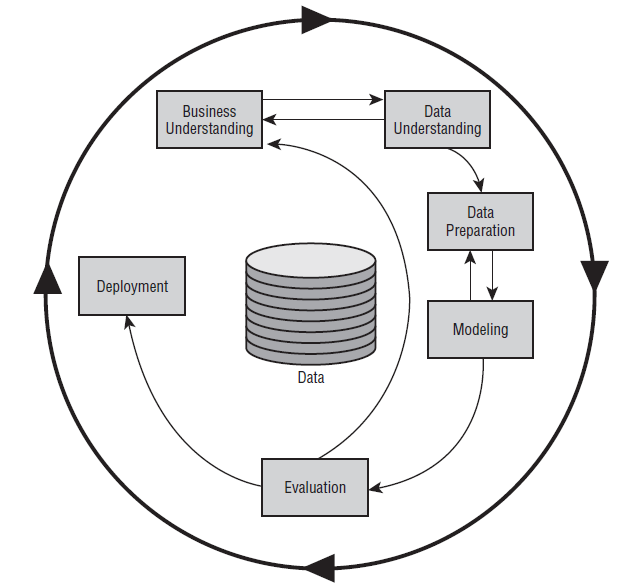
\includegraphics[width=.5\linewidth]{./images/crispdm}
    \caption{Ciclo di vita del CRISP-DM}	
\end{figure}

\bigskip

\begin{figure}[h!]
	\centering
    
\includegraphics{./images/kdd98}
    \caption{Logo di KDD Cup '98}
\end{figure}
	\clearpage
	\chapter[Business Understanding]{Business\\Understanding}
\label{ch:bisund}
In questo capitolo verrà affrontata la fase di Business Understanding, con l'individuazione degli obiettivi di business e le risorse per conseguirli.

\section{Background}
La competizione è supportata da un'organizzazione no-profit statunitense che fornisce programmi e servizi per i veterani americani che riportano ferite o malattie alla spina dorsale. Con un database interno di oltre 13 milioni di donatori, essa è anche uno dei più grandi organizzatori di raccolte fondi per corrispondenza nella nazione.

Nel 1997 è stata rinnovata la richiesta di fondi a chi aveva già fatto una donazione in precedenza. La mailing è stata mandata ad un totale di 3.5 milioni di donatori che erano presenti nel database a partire da giugno dello stesso anno.

Un gruppo che è di particolare interesse per questa organizzazione riguarda i \emph{Lapsed Donors}. Queste sono persone che hanno donato l'ultima volta 13 o 24 mesi fa. Rappresentano un gruppo importante, visto che più tempo passa da quando qualcuno fa una donazione, meno probabile sarà che lo farà di nuovo. Di conseguenza, ricatturare questi ex donatori è un aspetto importante per non vanificare gli sforzi della raccolta fondi messa in piedi dall'organizzazione.

\subsection{Risorse}

La popolazione per questa analisi riguarderà i Lapsed Donor che hanno ricevuto una lettera di sollecito nel giugno '97. Perciò il dataset d'analisi contiene un sottoinsieme dell'universo complessivo destinatario del mailing.

Il file comprende 95412 soggetti destinatari del mailing, con i rispondenti allo stesso segnalati con un flag nel campo \tb.

Il computer a disposizione è un HP Pavillion DV5-1105el con processore AMD Turion Dual-Core da 2,1 GHz e 4 GB di RAM. Il sistema operativo è Windows 8 Pro 64-bit.

Il software utilizzato nella sperimentazione è \textbf{Weka} (\textit{Waikato Environment for Knowledge Analysis}).

Il personale che lavora al progetto è formato solo dall'esaminando.

\subsection{Vincoli}
I detentori del data set hanno posto alcune condizioni per il suo utilizzo:
\begin{itemize}
	\item Il nome dell'organizzazione no-profit che ha fornito i dati deve rimanere anonima nel caso tali dati vengano utilizzati in futuro per nuove analisi.
	
	\item L'utente che sfrutterà i dati dovrà notificare ai dententori stessi:
	 	\begin{itemize}
	 	
		\item \texttt{Ismail Parsa (\href{mailto:iparsa@epsilon.com}{iparsa@epsilon.com})} e

		\item \texttt{Ken Howes (\href{mailto:khowes@epsilon.com}{khowes@epsilon.com})}
		
		\end{itemize}
	nel caso vengano prodotti risultati, grafici, tabelle, ecc. ed inviare una nota che includa una sintesi del risultato finale.

	\item Gli autori di articoli pubblicati e/o non pubblicati che usano il data set dovranno avvertire le persone suddette ed inviare una copia del loro lavoro.
\end{itemize}

La durata stimata del progetto è di 4 settimane.

\subsection{Presupposti}
Stando alle condizioni dettate sopra, i dati sono disponibili ai fini del progetto.

\section{Obiettivi di business}
Si vuole prevedere se un individuo effettuerà un'altra donazione in futuro.

\section{Criteri di successo}
Il processo KDD terminerà con successo se si riuscirà a costruire il miglior modello di predizione in termini di maggior copertura di istanze rispetto agli algoritmi standard, ottenuto confrontando varie tecniche di modellazione.

\section{Task di data mining}
Il task è di tipo \emph{predittivo} per l'attributo \tb{}; si tratterà di \emph{classificazione}, con lo scopo di etichettare i donatori contattati come possibili rispondenti o meno alla richiesta di fondi.

\section{Glossario}
\begin{itemize}
	\item Attributo = Campo = Variabile = Feature = Colonna
	\item Attributo target = Attributo di classe
	\item Osservazione = Esempio = Istanza = Riga
\end{itemize}

\section{Analisi costi-benefici}
I costi riguarderanno il tempo e le risorse computazionali utilizzati per perseguire gli obiettivi di business. I benefici riguarderanno invece l'individuazione di possibili rispondenti al sollecito della donazione che, appunto, daranno fondi all'associazione.

\section{Piano di progetto}
La maggior parte delle risorse temporali sono state utilizzate per lo studio e la preparazione del dataset per le successive elaborazioni, interessando quindi le fasi dal \nameref{ch:bisund}, \nameref{ch:datund} e \nameref{ch:datprep}, mentre le risorse computazionali hanno riguardato principalmente le fasi di \nameref{ch:model} ed \nameref{ch:eval} ed ancora la fase di \nameref{ch:datprep}. Si stima un tempo per l'ultimazione del progetto di 4 settimane.



	\clearpage
	\chapter{Data Understanding}
\label{ch:datund}
In questa fase verranno descritti e valutati i dati a disposizione.

\section{Raccolta dei dati}

Il dataset raccoglie i dati dei donatori inattivi che sono stati destinatari del mailing avvenuto nel giugno 1997. Esso è scaricabile dal sito del KDD Cup '98\footnote{\url{http://kdd.ics.uci.edu/databases/kddcup98/kddcup98.html}}.

\section{Descrizione dei dati}
Il training set contiene 95412 istanze corredate da 480 attributi, compreso l'attributo target. Quest'ultimo, \tb{}, etichetta i destinatari del mailing come potenziali donatori o meno. Può essere 0 se non è etichettato come donatore, 1 altrimenti.

Di seguito il resto degli attributi\footnote{Qui ne è presente una descrizione dettagliata: \url{http://kdd.ics.uci.edu/databases/kddcup98/epsilon_mirror/cup98dic.txt}}.


Questi attributi trattano informazioni di carattere generale sui donatori:
\begin{multicols}{3}
	\footnotesize
	\begin{verbatim}
		ODATEDW
		OSOURCE
		TCODE
		STATE
		ZIP
		MAILCODE
		PVASTATE
		DOB
		NOEXCH
		RECINHSE
		RECP3
		RECPGVG
		RECSWEEP
		MDMAUD
		DOMAIN
		CLUSTER
		AGE
		AGEFLAG
		HOMEOWNR
		CHILD03
		CHILD07
		CHILD12
		CHILD18
		NUMCHLD
		INCOME
		GENDER
		WEALTH1
		HIT
	\end{verbatim}
\end{multicols}

Gli attributi seguenti indicano il numero di volte in cui il donatore ha risposto ad altri tipi offerte per corrispondenza:

\begin{multicols}{3}
	\begin{verbatim}
		MBCRAFT
		MBGARDEN
		MBBOOKS
		MBCOLECT
		MAGFAML
		MAGFEM
		MAGMALE
		PUBGARDN
		PUBCULIN
		PUBHLTH
		PUBDOITY
		PUBNEWFN
		PUBPHOTO
		PUBOPP
	\end{verbatim}
\end{multicols}	

Gli attributi seguenti provengono da sorgenti di terze parti:
\begin{multicols}{3}
	\begin{verbatim}
		DATASRCE
		MALEMILI
		MALEVET
		VIETVETS
		WWIIVETS
		LOCALGOV
		STATEGOV
		FEDGOV
		SOLP3
		SOLIH
		MAJOR
		WEALTH2
		GEOCODE
	\end{verbatim}
\end{multicols}

Gli attributi seguenti riflettono gli interessi del donatore, che sono stati raccolti da sorgenti dati di terze parti:

\begin{multicols}{3}
	\begin{verbatim}
		COLLECT1
		VETERANS
		BIBLE
		CATLG
		HOMEE
		PETS
		CDPLAY
		STEREO
		PCOWNERS
		PHOTO
		CRAFTS
		FISHER
		GARDENIN
		BOATS
		WALKER
		KIDSTUFF
		CARDS
		PLATES
		LIFESRC
	\end{verbatim}
\end{multicols}

Gli attributi seguenti riflettono le caratteristiche del quartiere dei donatori, che sono state raccolte dal censimento degli USA del 1990:
\begin{multicols}{3}
	\begin{verbatim}
		PEPSTRFL
		POP901
		POP902
		POP903
		POP90C1
		POP90C2
		POP90C3
		POP90C4
		POP90C5
		ETH1
		ETH2
		ETH3
		ETH4
		ETH5
		ETH6
		ETH7
		ETH8
		ETH9
		ETH10
		ETH11
		ETH12
		ETH13
		ETH14
		ETH15
		ETH16
		AGE901
		AGE902
		AGE903
		AGE904
		AGE905
		AGE906
		AGE907
		CHIL1
		CHIL2
		CHIL3
		AGEC1
		AGEC2
		AGEC3
		AGEC4
		AGEC5
		AGEC6
		AGEC7
		CHILC1
		CHILC2
		CHILC3
		CHILC4
		CHILC5
		HHAGE1
		HHAGE2
		HHAGE3
		HHN1
		HHN2
		HHN3
		HHN4
		HHN5
		HHN6
		MARR1
		MARR2
		MARR3
		MARR4
		HHP1
		HHP2
		DW1
		DW2
		DW3
		DW4
		DW5
		DW6
		DW7
		DW8
		DW9
		HV1
		HV2
		HV3
		HV4
		HU1
		HU2
		HU3
		HU4
		HU5
		HHD1
		HHD2
		HHD3
		HHD4
		HHD5
		HHD6
		HHD7
		HHD8
		HHD9
		HHD10
		HHD11
		HHD12
		ETHC1
		ETHC2
		ETHC3
		ETHC4
		ETHC5
		ETHC6
		HVP1
		HVP2
		HVP3
		HVP4
		HVP5
		HVP6
		HUR1
		HUR2
		RHP1
		RHP2
		RHP3
		RHP4
		HUPA1
		HUPA2
		HUPA3
		HUPA4
		HUPA5
		HUPA6
		HUPA7
		RP1
		RP2
		RP3
		RP4
		MSA
		ADI
		DMA
		IC1
		IC2
		IC3
		IC4
		IC5
		IC6
		IC7
		IC8
		IC9
		IC10
		IC11
		IC12
		IC13
		IC14
		IC15
		IC16
		IC17
		IC18
		IC19
		IC20
		IC21
		IC22
		IC23
		HHAS1
		HHAS2
		HHAS3
		HHAS4
		MC1
		MC2
		MC3
		TPE1
		TPE2
		TPE3
		TPE4
		TPE5
		TPE6
		TPE7
		TPE8
		TPE9
		PEC1
		PEC2
		TPE10
		TPE11
		TPE12
		TPE13
		LFC1
		LFC2
		LFC3
		LFC4
		LFC5
		LFC6
		LFC7
		LFC8
		LFC9
		LFC10
		OCC1
		OCC2
		OCC3
		OCC4
		OCC5
		OCC6
		OCC7
		OCC8
		OCC9
		OCC10
		OCC11
		OCC12
		OCC13
		EIC1
		EIC2
		EIC3
		EIC4
		EIC5
		EIC6
		EIC7
		EIC8
		EIC9
		EIC10
		EIC11
		EIC12
		EIC13
		EIC14
		EIC15
		EIC16
		OEDC1
		OEDC2
		OEDC3
		OEDC4
		OEDC5
		OEDC6
		OEDC7
		EC1
		EC2
		EC3
		EC4
		EC5
		EC6
		EC7
		EC8
		SEC1
		SEC2
		SEC3
		SEC4
		SEC5
		AFC1
		AFC2
		AFC3
		AFC4
		AFC5
		AFC6
		VC1
		VC2
		VC3
		VC4
		ANC1
		ANC2
		ANC3
		ANC4
		ANC5
		ANC6
		ANC7
		ANC8
		ANC9
		ANC10
		ANC11
		ANC12
		ANC13
		ANC14
		ANC15
		POBC1
		POBC2
		LSC1
		LSC2
		LSC3
		LSC4
		VOC1
		VOC2
		VOC3
		HC1
		HC2
		HC3
		HC4
		HC5
		HC6
		HC7
		HC8
		HC9
		HC10
		HC11
		HC12
		HC13
		HC14
		HC15
		HC16
		HC17
		HC18
		HC19
		HC20
		HC21
		MHUC1
		MHUC2
		AC1
		AC2
	\end{verbatim}
\end{multicols}		

Gli attributi seguenti provengono dal file dello storico delle promozioni:

\begin{multicols}{3}
	\begin{verbatim}
		ADATE_2
		ADATE_3
		ADATE_4
		ADATE_5
		ADATE_6
		ADATE_7
		ADATE_8
		ADATE_9
		ADATE_10
		ADATE_11
		ADATE_12
		ADATE_13
		ADATE_14
		ADATE_15
		ADATE_16
		ADATE_17
		ADATE_18
		ADATE_19
		ADATE_20
		ADATE_21
		ADATE_22
		ADATE_23
		ADATE_24
		RFA_2
		RFA_3
		RFA_4
		RFA_5
		RFA_6
		RFA_7
		RFA_8
		RFA_9
		RFA_10
		RFA_11
		RFA_12
		RFA_13
		RFA_14
		RFA_15
		RFA_16
		RFA_17
		RFA_18
		RFA_19
		RFA_20
		RFA_21
		RFA_22
		RFA_23
		RFA_24
	\end{verbatim}
\end{multicols}

Gli attributi seguenti sono variabili aggregate, ricavate dallo storico delle promozioni:
\begin{multicols}{3}
	\begin{verbatim}
		CARDPROM
		MAXADATE
		NUMPROM
		CARDPM12
		NUMPRM12
	\end{verbatim}
\end{multicols}

Gli attributi seguenti sono altre variabili provenienti dallo storico delle promozioni:

\begin{multicols}{3}
	\begin{verbatim}
		RDATE_3
		RDATE_4
		RDATE_5
		RDATE_6
		RDATE_7
		RDATE_8
		RDATE_9
		RDATE_10
		RDATE_11
		RDATE_12
		RDATE_13
		RDATE_14
		RDATE_15
		RDATE_16
		RDATE_17
		RDATE_18
		RDATE_19
		RDATE_20
		RDATE_21
		RDATE_22
		RDATE_23
		RDATE_24
		RAMNT_3
		RAMNT_4
		RAMNT_5
		RAMNT_6
		RAMNT_7
		RAMNT_8
		RAMNT_9
		RAMNT_10
		RAMNT_11
		RAMNT_12
		RAMNT_13
		RAMNT_14
		RAMNT_15
		RAMNT_16
		RAMNT_17
		RAMNT_18
		RAMNT_19
		RAMNT_20
		RAMNT_21
		RAMNT_22
		RAMNT_23
		RAMNT_24
	\end{verbatim}
\end{multicols}

Gli attributi seguenti sono altre variabili aggregate, sempre ricavate dallo storico delle promozioni:

\begin{multicols}{3}
	\begin{verbatim}
		RAMNTALL
		NGIFTALL
		CARDGIFT
		MINRAMNT
		MINRDATE
		MAXRAMNT
		MAXRDATE
		LASTGIFT
		LASTDATE
		FISTDATE
		NEXTDATE
		TIMELAG
		AVGGIFT
	\end{verbatim}
\end{multicols}

Di seguito il resto degli attributi, compresi quelli target:
\begin{multicols}{3}
	\begin{verbatim}	
		CONTROLN
		TARGET_B
		HPHONE_D
		RFA_2R
		RFA_2F
		RFA_2A
		MDMAUD_R
		MDMAUD_F
		MDMAUD_A
		CLUSTER2
		GEOCODE2
	\end{verbatim}
\end{multicols}

Gli attributi ricadono in tutte le categorie esistenti, quindi ce ne sono di \emph{nominali} (es. \texttt{TCODE}, che raccoglie i codici che indicano i titoli dei donatori), \emph{ordinali} (es. \texttt{WEIGHT2}, che rappresenta un indice di ricchezza che va da 0, il più basso, a 9, il più alto), \emph{interi} (es. \texttt{POP901}, il numero di persone) e \emph{continu}i (es. \texttt{POP90C4}, la percentuale di maschi).

Le istanze presentano un notevole sbilanciamento nei valori dell'attributo \tb, in quanto il valore 0 è presente nel 94,9\%, mentre il valore 1 solo il 5,1\%.

\section{Verifica della qualità dei dati}
In questa sezione vengono analizzati i seguenti aspetti relativi alla qualità dei dati:

\begin{itemize}
	\item \textbf{Accuratezza}: I valori memorizzati riflettono i dati reali, quindi sono da ritenersi accurati.
	\item \textbf{Completezza}: Alcune istanze presentano dei valori mancanti, quindi non sono complete.
	\item \textbf{Consistenza}: I dati sono rappresentati in maniera uniforme nel dataset.
	\item \textbf{Attualità}: I dati furono raccolti nel giugno '97 per il KDD Cup '98, quindi si dimostrarono aggiornati per gli scopi della competizione.
\end{itemize}

\section{Esplorazione dei dati}
Di seguito le caratteristiche degli attributi:
% latex table generated in R 3.1.2 by xtable 1.7-4 package
% Thu Jan 08 14:40:33 2015
\setlength\LTleft{-1.5cm}
\setlength\LTright{-1.5cm}
\setlength{\tabcolsep}{0.15cm}
\begin{longtable}{|rrrrrrrrr|}
	\hline
	& missing &  min  &  max  &  median  &  mean  &  var  &  std.dev& \\
	\hline
	AGE  &  23665  &  1.00  &  98.00  &  62.00  &  61.61  &  277.70  &  16.66 & \\
	NUMCHLD  &  83026  &  1.00  &  7.00  &  1.00  &  1.53  &  0.65  &  0.81 & \\
	INCOME  &  21286  &  1.00  &  7.00  &  4.00  &  3.89  &  3.44  &  1.85 & \\
	WEALTH1  &  44732  &  0.00  &  9.00  &  6.00  &  5.35  &  7.52  &  2.74 & \\
	HIT  &  0  &  0.00  &  241.00  &  0.00  &  3.32  &  86.62  &  9.31 & \\
	MBCRAFT  &  52854  &  0.00  &  6.00  &  0.00  &  0.15  &  0.22  &  0.47 & \\
	MBGARDEN  &  52854  &  0.00  &  4.00  &  0.00  &  0.06  &  0.07  &  0.26 & \\
	MBBOOKS  &  52854  &  0.00  &  9.00  &  0.00  &  1.12  &  2.79  &  1.67 & \\
	MBCOLECT  &  52914  &  0.00  &  6.00  &  0.00  &  0.06  &  0.09  &  0.30 & \\
	MAGFAML  &  52854  &  0.00  &  9.00  &  0.00  &  0.45  &  0.67  &  0.82 & \\
	MAGFEM  &  52854  &  0.00  &  5.00  &  0.00  &  0.13  &  0.15  &  0.38 & \\
	MAGMALE  &  52854  &  0.00  &  4.00  &  0.00  &  0.07  &  0.08  &  0.28 & \\
	PUBGARDN  &  52854  &  0.00  &  5.00  &  0.00  &  0.14  &  0.24  &  0.49 & \\
	PUBCULIN  &  52854  &  0.00  &  6.00  &  0.00  &  0.15  &  0.18  &  0.43 & \\
	PUBHLTH  &  52854  &  0.00  &  9.00  &  0.00  &  0.71  &  1.56  &  1.25 & \\
	PUBDOITY  &  52854  &  0.00  &  8.00  &  0.00  &  0.24  &  0.53  &  0.73 & \\
	PUBNEWFN  &  52854  &  0.00  &  9.00  &  0.00  &  0.38  &  0.92  &  0.96 & \\
	PUBPHOTO  &  52854  &  0.00  &  2.00  &  0.00  &  0.01  &  0.01  &  0.08 & \\
	PUBOPP  &  52854  &  0.00  &  9.00  &  0.00  &  0.24  &  0.77  &  0.88 & \\
	MALEMILI  &  0  &  0.00  &  99.00  &  0.00  &  1.05  &  25.66  &  5.07 & \\
	MALEVET  &  0  &  0.00  &  99.00  &  31.00  &  30.45  &  131.57  &  11.47 & \\
	VIETVETS  &  0  &  0.00  &  99.00  &  29.00  &  29.70  &  227.94  &  15.10 & \\
	WWIIVETS  &  0  &  0.00  &  99.00  &  32.00  &  32.64  &  313.61  &  17.71 & \\
	LOCALGOV  &  0  &  0.00  &  99.00  &  6.00  &  6.84  &  19.29  &  4.39 & \\
	STATEGOV  &  0  &  0.00  &  99.00  &  3.00  &  4.57  &  26.28  &  5.13 & \\
	FEDGOV  &  0  &  0.00  &  87.00  &  2.00  &  3.11  &  17.27  &  4.16 & \\
	WEALTH2  &  43823  &  0.00  &  9.00  &  5.00  &  4.95  &  7.86  &  2.80 & \\
	POP901  &  0  &  0.00  &  98701.00  &  1565.00  &  3255.88  &  32984544.57  &  5743.22 & \\
	POP902  &  0  &  0.00  &  23766.00  &  421.00  &  864.99  &  2126065.63  &  1458.10 & \\
	POP903  &  0  &  0.00  &  35403.00  &  585.00  &  1222.57  &  4507537.65  &  2123.10 & \\
	POP90C1  &  0  &  0.00  &  99.00  &  99.00  &  58.59  &  2249.68  &  47.43 & \\
	POP90C2  &  0  &  0.00  &  99.00  &  0.00  &  13.62  &  974.82  &  31.22 & \\
	POP90C3  &  0  &  0.00  &  99.00  &  0.00  &  26.14  &  1603.03  &  40.04 & \\
	POP90C4  &  0  &  0.00  &  99.00  &  49.00  &  48.21  &  30.98  &  5.57 & \\
	POP90C5  &  0  &  0.00  &  99.00  &  51.00  &  50.95  &  33.27  &  5.77 & \\
	ETH1  &  0  &  0.00  &  99.00  &  93.00  &  84.85  &  441.58  &  21.01 & \\
	ETH2  &  0  &  0.00  &  99.00  &  1.00  &  7.47  &  278.58  &  16.69 & \\
	ETH3  &  0  &  0.00  &  99.00  &  0.00  &  0.78  &  12.04  &  3.47 & \\
	ETH4  &  0  &  0.00  &  99.00  &  1.00  &  2.91  &  49.98  &  7.07 & \\
	ETH5  &  0  &  0.00  &  99.00  &  2.00  &  7.46  &  190.06  &  13.79 & \\
	ETH6  &  0  &  0.00  &  22.00  &  0.00  &  0.22  &  0.46  &  0.68 & \\
	ETH7  &  0  &  0.00  &  72.00  &  0.00  &  0.40  &  4.98  &  2.23 & \\
	ETH8  &  0  &  0.00  &  99.00  &  0.00  &  0.61  &  6.42  &  2.53 & \\
	ETH9  &  0  &  0.00  &  67.00  &  0.00  &  0.56  &  5.33  &  2.31 & \\
	ETH10  &  0  &  0.00  &  46.00  &  0.00  &  0.25  &  1.01  &  1.00 & \\
	ETH11  &  0  &  0.00  &  47.00  &  0.00  &  0.21  &  1.11  &  1.05 & \\
	ETH12  &  0  &  0.00  &  72.00  &  0.00  &  0.07  &  1.37  &  1.17 & \\
	ETH13  &  0  &  0.00  &  97.00  &  1.00  &  5.14  &  128.45  &  11.33 & \\
	ETH14  &  0  &  0.00  &  57.00  &  0.00  &  0.30  &  1.67  &  1.29 & \\
	ETH15  &  0  &  0.00  &  81.00  &  0.00  &  0.33  &  10.30  &  3.21 & \\
	ETH16  &  0  &  0.00  &  86.00  &  1.00  &  1.51  &  11.33  &  3.37 & \\
	AGE901  &  0  &  0.00  &  84.00  &  33.00  &  34.48  &  69.48  &  8.34 & \\
	AGE902  &  0  &  0.00  &  84.00  &  41.00  &  41.91  &  68.06  &  8.25 & \\
	AGE903  &  0  &  0.00  &  84.00  &  44.00  &  45.11  &  65.76  &  8.11 & \\
	AGE904  &  0  &  0.00  &  84.00  &  35.00  &  35.92  &  52.73  &  7.26 & \\
	AGE905  &  0  &  0.00  &  84.00  &  45.00  &  44.69  &  48.44  &  6.96 & \\
	AGE906  &  0  &  0.00  &  84.00  &  48.00  &  47.89  &  47.37  &  6.88 & \\
	AGE907  &  0  &  0.00  &  75.00  &  26.00  &  24.52  &  56.48  &  7.52 & \\
	CHIL1  &  0  &  0.00  &  99.00  &  39.00  &  39.59  &  67.77  &  8.23 & \\
	CHIL2  &  0  &  0.00  &  99.00  &  39.00  &  38.36  &  40.71  &  6.38 & \\
	CHIL3  &  0  &  0.00  &  99.00  &  21.00  &  21.01  &  33.96  &  5.83 & \\
	AGEC1  &  0  &  0.00  &  99.00  &  11.00  &  12.20  &  36.82  &  6.07 & \\
	AGEC2  &  0  &  0.00  &  99.00  &  22.00  &  22.19  &  60.65  &  7.79 & \\
	AGEC3  &  0  &  0.00  &  99.00  &  20.00  &  20.65  &  38.58  &  6.21 & \\
	AGEC4  &  0  &  0.00  &  99.00  &  14.00  &  14.06  &  18.63  &  4.32 & \\
	AGEC5  &  0  &  0.00  &  99.00  &  12.00  &  11.86  &  17.19  &  4.15 & \\
	AGEC6  &  0  &  0.00  &  99.00  &  10.00  &  10.54  &  36.05  &  6.00 & \\
	AGEC7  &  0  &  0.00  &  99.00  &  6.00  &  7.67  &  45.21  &  6.72 & \\
	CHILC1  &  0  &  0.00  &  99.00  &  16.00  &  16.18  &  26.22  &  5.12 & \\
	CHILC2  &  0  &  0.00  &  99.00  &  16.00  &  16.14  &  13.66  &  3.70 & \\
	CHILC3  &  0  &  0.00  &  99.00  &  32.00  &  31.63  &  28.99  &  5.38 & \\
	CHILC4  &  0  &  0.00  &  99.00  &  20.00  &  19.75  &  20.81  &  4.56 & \\
	CHILC5  &  0  &  0.00  &  99.00  &  15.00  &  15.26  &  31.84  &  5.64 & \\
	HHAGE1  &  0  &  0.00  &  99.00  &  23.00  &  24.60  &  171.36  &  13.09 & \\
	HHAGE2  &  0  &  0.00  &  99.00  &  8.00  &  9.37  &  55.38  &  7.44 & \\
	HHAGE3  &  0  &  0.00  &  99.00  &  21.00  &  22.31  &  168.06  &  12.96 & \\
	HHN1  &  0  &  0.00  &  99.00  &  21.00  &  22.82  &  138.52  &  11.77 & \\
	HHN2  &  0  &  0.00  &  99.00  &  33.00  &  33.63  &  67.77  &  8.23 & \\
	HHN3  &  0  &  0.00  &  99.00  &  44.00  &  42.70  &  211.37  &  14.54 & \\
	HHN4  &  0  &  0.00  &  99.00  &  26.00  &  25.62  &  122.31  &  11.06 & \\
	HHN5  &  0  &  0.00  &  99.00  &  10.00  &  10.47  &  40.74  &  6.38 & \\
	HHN6  &  0  &  0.00  &  99.00  &  3.00  &  3.90  &  14.39  &  3.79 & \\
	MARR1  &  0  &  0.00  &  99.00  &  61.00  &  58.10  &  168.16  &  12.97 & \\
	MARR2  &  0  &  0.00  &  99.00  &  10.00  &  10.69  &  20.46  &  4.52 & \\
	MARR3  &  0  &  0.00  &  73.00  &  6.00  &  7.42  &  23.89  &  4.89 & \\
	MARR4  &  0  &  0.00  &  99.00  &  21.00  &  22.95  &  78.90  &  8.88 & \\
	HHP1  &  0  &  0.00  &  650.00  &  182.00  &  185.27  &  2504.12  &  50.04 & \\
	HHP2  &  0  &  0.00  &  700.00  &  262.00  &  259.68  &  2490.19  &  49.90 & \\
	DW1  &  0  &  0.00  &  99.00  &  75.00  &  70.08  &  623.73  &  24.97 & \\
	DW2  &  0  &  0.00  &  99.00  &  72.00  &  66.04  &  694.49  &  26.35 & \\
	DW3  &  0  &  0.00  &  99.00  &  1.00  &  2.90  &  28.79  &  5.37 & \\
	DW4  &  0  &  0.00  &  99.00  &  9.00  &  19.48  &  569.03  &  23.85 & \\
	DW5  &  0  &  0.00  &  99.00  &  6.00  &  16.56  &  512.82  &  22.65 & \\
	DW6  &  0  &  0.00  &  99.00  &  3.00  &  13.10  &  418.52  &  20.46 & \\
	DW7  &  0  &  0.00  &  99.00  &  0.00  &  1.79  &  34.89  &  5.91 & \\
	DW8  &  0  &  0.00  &  99.00  &  0.00  &  1.16  &  18.10  &  4.25 & \\
	DW9  &  0  &  0.00  &  99.00  &  0.00  &  0.62  &  15.76  &  3.97 & \\
	HV1  &  0  &  0.00  &  6000.00  &  737.00  &  1061.84  &  886923.00  &  941.77 & \\
	HV2  &  0  &  0.00  &  6000.00  &  803.00  &  1133.03  &  897537.61  &  947.38 & \\
	HV3  &  0  &  0.00  &  13.00  &  4.00  &  4.22  &  5.33  &  2.31 & \\
	HV4  &  0  &  0.00  &  13.00  &  3.00  &  3.88  &  5.04  &  2.24 & \\
	HU1  &  0  &  0.00  &  99.00  &  76.00  &  69.70  &  471.63  &  21.72 & \\
	HU2  &  0  &  0.00  &  99.00  &  24.00  &  29.45  &  436.82  &  20.90 & \\
	HU3  &  0  &  0.00  &  99.00  &  94.00  &  89.97  &  167.84  &  12.96 & \\
	HU4  &  0  &  0.00  &  99.00  &  6.00  &  9.18  &  99.22  &  9.96 & \\
	HU5  &  0  &  0.00  &  99.00  &  5.00  &  13.74  &  440.23  &  20.98 & \\
	HHD1  &  0  &  0.00  &  99.00  &  36.00  &  35.65  &  169.91  &  13.04 & \\
	HHD2  &  0  &  0.00  &  99.00  &  75.00  &  71.50  &  229.12  &  15.14 & \\
	HHD3  &  0  &  0.00  &  99.00  &  61.00  &  58.76  &  263.72  &  16.24 & \\
	HHD4  &  0  &  0.00  &  99.00  &  28.00  &  27.78  &  142.60  &  11.94 & \\
	HHD5  &  0  &  0.00  &  99.00  &  86.00  &  81.93  &  199.00  &  14.11 & \\
	HHD6  &  0  &  0.00  &  99.00  &  14.00  &  17.24  &  144.75  &  12.03 & \\
	HHD7  &  0  &  0.00  &  99.00  &  7.00  &  7.87  &  28.06  &  5.30 & \\
	HHD8  &  0  &  0.00  &  50.00  &  1.00  &  1.62  &  1.26  &  1.12 & \\
	HHD9  &  0  &  0.00  &  99.00  &  5.00  &  6.25  &  21.93  &  4.68 & \\
	HHD10  &  0  &  0.00  &  99.00  &  12.00  &  13.61  &  50.46  &  7.10 & \\
	HHD11  &  0  &  0.00  &  99.00  &  18.00  &  18.91  &  87.53  &  9.36 & \\
	HHD12  &  0  &  0.00  &  99.00  &  4.00  &  4.82  &  17.00  &  4.12 & \\
	ETHC1  &  0  &  0.00  &  75.00  &  18.00  &  16.75  &  47.09  &  6.86 & \\
	ETHC2  &  0  &  0.00  &  99.00  &  55.00  &  50.79  &  210.94  &  14.52 & \\
	ETHC3  &  0  &  0.00  &  99.00  &  15.00  &  17.36  &  151.27  &  12.30 & \\
	ETHC4  &  0  &  0.00  &  55.00  &  0.00  &  1.96  &  20.68  &  4.55 & \\
	ETHC5  &  0  &  0.00  &  99.00  &  1.00  &  4.57  &  101.47  &  10.07 & \\
	ETHC6  &  0  &  0.00  &  99.00  &  0.00  &  0.84  &  8.52  &  2.92 & \\
	HVP1  &  0  &  0.00  &  99.00  &  1.00  &  13.59  &  708.79  &  26.62 & \\
	HVP2  &  0  &  0.00  &  99.00  &  3.00  &  21.05  &  1017.46  &  31.90 & \\
	HVP3  &  0  &  0.00  &  99.00  &  17.00  &  35.11  &  1342.84  &  36.64 & \\
	HVP4  &  0  &  0.00  &  99.00  &  48.00  &  51.17  &  1350.20  &  36.75 & \\
	HVP5  &  0  &  0.00  &  99.00  &  89.00  &  73.91  &  875.93  &  29.60 & \\
	HVP6  &  0  &  0.00  &  99.00  &  0.00  &  6.45  &  326.34  &  18.06 & \\
	HUR1  &  0  &  0.00  &  99.00  &  2.00  &  4.85  &  56.93  &  7.55 & \\
	HUR2  &  0  &  0.00  &  99.00  &  44.00  &  45.75  &  459.63  &  21.44 & \\
	RHP1  &  0  &  0.00  &  85.00  &  52.00  &  52.94  &  115.24  &  10.73 & \\
	RHP2  &  0  &  0.00  &  90.00  &  54.00  &  53.77  &  108.47  &  10.41 & \\
	RHP3  &  0  &  0.00  &  61.00  &  14.00  &  14.14  &  6.55  &  2.56 & \\
	RHP4  &  0  &  0.00  &  40.00  &  4.00  &  4.39  &  1.40  &  1.18 & \\
	HUPA1  &  0  &  0.00  &  99.00  &  5.00  &  10.15  &  163.59  &  12.79 & \\
	HUPA2  &  0  &  0.00  &  99.00  &  1.00  &  9.31  &  292.73  &  17.11 & \\
	HUPA3  &  0  &  0.00  &  99.00  &  0.00  &  8.55  &  207.46  &  14.40 & \\
	HUPA4  &  0  &  0.00  &  99.00  &  10.00  &  11.16  &  60.77  &  7.80 & \\
	HUPA5  &  0  &  0.00  &  99.00  &  2.00  &  5.22  &  55.65  &  7.46 & \\
	HUPA6  &  0  &  0.00  &  99.00  &  2.00  &  11.01  &  317.13  &  17.81 & \\
	HUPA7  &  0  &  0.00  &  99.00  &  0.00  &  1.61  &  9.13  &  3.02 & \\
	RP1  &  0  &  0.00  &  99.00  &  14.00  &  29.14  &  1036.53  &  32.20 & \\
	RP2  &  0  &  0.00  &  99.00  &  36.00  &  42.37  &  1220.16  &  34.93 & \\
	RP3  &  0  &  0.00  &  99.00  &  68.00  &  59.68  &  1082.01  &  32.89 & \\
	RP4  &  0  &  0.00  &  99.00  &  86.00  &  76.52  &  589.32  &  24.28 & \\
	MSA  &  132  &  0.00  &  9360.00  &  3350.00  &  3527.74  &  8201950.34  &  2863.90 & \\
	ADI  &  132  &  0.00  &  651.00  &  175.00  &  187.36  &  18774.26  &  137.02 & \\
	DMA  &  132  &  0.00  &  881.00  &  635.00  &  664.00  &  13540.49  &  116.36 & \\
	IC1  &  0  &  0.00  &  1500.00  &  310.00  &  340.06  &  26530.96  &  162.88 & \\
	IC2  &  0  &  0.00  &  1500.00  &  355.00  &  387.03  &  30142.04  &  173.61 & \\
	IC3  &  0  &  0.00  &  1500.00  &  354.00  &  387.42  &  26008.25  &  161.27 & \\
	IC4  &  0  &  0.00  &  1500.00  &  397.00  &  430.79  &  29461.43  &  171.64 & \\
	IC5  &  0  &  0.00  &  174523.00  &  13727.50  &  15722.74  &  73336046.10  &  8563.65 & \\
	IC6  &  0  &  0.00  &  99.00  &  19.00  &  21.50  &  210.56  &  14.51 & \\
	IC7  &  0  &  0.00  &  99.00  &  17.00  &  16.91  &  63.35  &  7.96 & \\
	IC8  &  0  &  0.00  &  99.00  &  16.00  &  15.75  &  39.42  &  6.28 & \\
	IC9  &  0  &  0.00  &  99.00  &  18.00  &  18.34  &  55.32  &  7.44 & \\
	IC10  &  0  &  0.00  &  99.00  &  15.00  &  15.95  &  93.82  &  9.69 & \\
	IC11  &  0  &  0.00  &  99.00  &  4.00  &  5.59  &  34.05  &  5.84 & \\
	IC12  &  0  &  0.00  &  50.00  &  1.00  &  2.21  &  11.20  &  3.35 & \\
	IC13  &  0  &  0.00  &  61.00  &  0.00  &  0.94  &  3.70  &  1.92 & \\
	IC14  &  0  &  0.00  &  99.00  &  0.00  &  1.89  &  21.54  &  4.64 & \\
	IC15  &  0  &  0.00  &  99.00  &  12.00  &  14.80  &  152.30  &  12.34 & \\
	IC16  &  0  &  0.00  &  99.00  &  16.00  &  15.93  &  84.10  &  9.17 & \\
	IC17  &  0  &  0.00  &  99.00  &  17.00  &  16.43  &  58.38  &  7.64 & \\
	IC18  &  0  &  0.00  &  99.00  &  21.00  &  20.61  &  71.79  &  8.47 & \\
	IC19  &  0  &  0.00  &  99.00  &  18.00  &  18.67  &  113.30  &  10.64 & \\
	IC20  &  0  &  0.00  &  99.00  &  4.00  &  6.58  &  44.44  &  6.67 & \\
	IC21  &  0  &  0.00  &  50.00  &  1.00  &  2.60  &  15.27  &  3.91 & \\
	IC22  &  0  &  0.00  &  99.00  &  0.00  &  1.12  &  5.39  &  2.32 & \\
	IC23  &  0  &  0.00  &  99.00  &  0.00  &  2.28  &  30.60  &  5.53 & \\
	HHAS1  &  0  &  0.00  &  99.00  &  26.00  &  26.76  &  192.24  &  13.86 & \\
	HHAS2  &  0  &  0.00  &  99.00  &  4.00  &  6.10  &  38.63  &  6.22 & \\
	HHAS3  &  0  &  0.00  &  99.00  &  43.00  &  42.96  &  290.85  &  17.05 & \\
	HHAS4  &  0  &  0.00  &  99.00  &  8.00  &  10.74  &  99.35  &  9.97 & \\
	MC1  &  0  &  0.00  &  99.00  &  47.00  &  48.36  &  255.25  &  15.98 & \\
	MC2  &  0  &  0.00  &  99.00  &  53.00  &  50.75  &  257.43  &  16.04 & \\
	MC3  &  0  &  0.00  &  99.00  &  10.00  &  12.28  &  105.17  &  10.26 & \\
	TPE1  &  0  &  0.00  &  99.00  &  79.00  &  76.10  &  176.62  &  13.29 & \\
	TPE2  &  0  &  0.00  &  99.00  &  12.00  &  13.00  &  44.86  &  6.70 & \\
	TPE3  &  0  &  0.00  &  99.00  &  0.00  &  2.40  &  31.26  &  5.59 & \\
	TPE4  &  0  &  0.00  &  99.00  &  0.00  &  1.83  &  20.95  &  4.58 & \\
	TPE5  &  0  &  0.00  &  71.00  &  0.00  &  0.45  &  4.83  &  2.20 & \\
	TPE6  &  0  &  0.00  &  47.00  &  0.00  &  0.10  &  0.54  &  0.73 & \\
	TPE7  &  0  &  0.00  &  25.00  &  0.00  &  0.24  &  0.48  &  0.70 & \\
	TPE8  &  0  &  0.00  &  99.00  &  3.00  &  4.07  &  30.17  &  5.49 & \\
	TPE9  &  0  &  0.00  &  99.00  &  2.00  &  3.25  &  13.60  &  3.69 & \\
	PEC1  &  0  &  0.00  &  99.00  &  1.00  &  2.27  &  38.88  &  6.24 & \\
	PEC2  &  0  &  0.00  &  99.00  &  11.00  &  18.30  &  363.19  &  19.06 & \\
	TPE10  &  0  &  0.00  &  90.00  &  19.00  &  19.48  &  45.87  &  6.77 & \\
	TPE11  &  0  &  0.00  &  76.00  &  23.00  &  23.72  &  43.96  &  6.63 & \\
	TPE12  &  0  &  0.00  &  99.00  &  4.00  &  5.31  &  28.55  &  5.34 & \\
	TPE13  &  0  &  0.00  &  99.00  &  64.00  &  60.04  &  302.81  &  17.40 & \\
	LFC1  &  0  &  0.00  &  99.00  &  66.00  &  64.53  &  185.00  &  13.60 & \\
	LFC2  &  0  &  0.00  &  99.00  &  76.00  &  73.85  &  214.43  &  14.64 & \\
	LFC3  &  0  &  0.00  &  99.00  &  57.00  &  56.02  &  188.84  &  13.74 & \\
	LFC4  &  0  &  0.00  &  99.00  &  72.00  &  69.80  &  224.49  &  14.98 & \\
	LFC5  &  0  &  0.00  &  99.00  &  54.00  &  52.96  &  188.85  &  13.74 & \\
	LFC6  &  0  &  0.00  &  99.00  &  66.00  &  64.11  &  268.63  &  16.39 & \\
	LFC7  &  0  &  0.00  &  99.00  &  50.00  &  48.80  &  298.68  &  17.28 & \\
	LFC8  &  0  &  0.00  &  99.00  &  78.00  &  70.10  &  946.68  &  30.77 & \\
	LFC9  &  0  &  0.00  &  99.00  &  97.00  &  62.66  &  1999.95  &  44.72 & \\
	LFC10  &  0  &  0.00  &  99.00  &  4.00  &  6.64  &  85.55  &  9.25 & \\
	OCC1  &  0  &  0.00  &  99.00  &  13.00  &  14.12  &  67.76  &  8.23 & \\
	OCC2  &  0  &  0.00  &  99.00  &  11.00  &  12.60  &  50.96  &  7.14 & \\
	OCC3  &  0  &  0.00  &  99.00  &  3.00  &  3.54  &  6.58  &  2.57 & \\
	OCC4  &  0  &  0.00  &  99.00  &  12.00  &  12.40  &  30.69  &  5.54 & \\
	OCC5  &  0  &  0.00  &  99.00  &  15.00  &  15.50  &  32.91  &  5.74 & \\
	OCC6  &  0  &  0.00  &  43.00  &  0.00  &  0.42  &  0.99  &  1.00 & \\
	OCC7  &  0  &  0.00  &  55.00  &  1.00  &  1.64  &  3.55  &  1.89 & \\
	OCC8  &  0  &  0.00  &  99.00  &  10.00  &  10.54  &  36.33  &  6.03 & \\
	OCC9  &  0  &  0.00  &  99.00  &  1.00  &  2.86  &  26.08  &  5.11 & \\
	OCC10  &  0  &  0.00  &  99.00  &  11.00  &  11.38  &  34.33  &  5.86 & \\
	OCC11  &  0  &  0.00  &  99.00  &  5.00  &  6.31  &  34.51  &  5.87 & \\
	OCC12  &  0  &  0.00  &  99.00  &  4.00  &  4.01  &  10.39  &  3.22 & \\
	OCC13  &  0  &  0.00  &  99.00  &  3.00  &  3.74  &  8.88  &  2.98 & \\
	EIC1  &  0  &  0.00  &  99.00  &  1.00  &  3.16  &  31.03  &  5.57 & \\
	EIC2  &  0  &  0.00  &  65.00  &  0.00  &  0.72  &  6.06  &  2.46 & \\
	EIC3  &  0  &  0.00  &  99.00  &  6.00  &  6.41  &  16.99  &  4.12 & \\
	EIC4  &  0  &  0.00  &  99.00  &  15.00  &  16.97  &  103.37  &  10.17 & \\
	EIC5  &  0  &  0.00  &  99.00  &  4.00  &  4.28  &  10.25  &  3.20 & \\
	EIC6  &  0  &  0.00  &  64.00  &  2.00  &  2.71  &  5.45  &  2.34 & \\
	EIC7  &  0  &  0.00  &  99.00  &  4.00  &  4.37  &  9.59  &  3.10 & \\
	EIC8  &  0  &  0.00  &  99.00  &  17.00  &  16.92  &  38.18  &  6.18 & \\
	EIC9  &  0  &  0.00  &  99.00  &  6.00  &  6.86  &  21.72  &  4.66 & \\
	EIC10  &  0  &  0.00  &  99.00  &  4.00  &  4.68  &  9.45  &  3.07 & \\
	EIC11  &  0  &  0.00  &  99.00  &  3.00  &  3.29  &  10.42  &  3.23 & \\
	EIC12  &  0  &  0.00  &  67.00  &  1.00  &  1.55  &  4.98  &  2.23 & \\
	EIC13  &  0  &  0.00  &  99.00  &  8.00  &  8.05  &  20.22  &  4.50 & \\
	EIC14  &  0  &  0.00  &  99.00  &  7.00  &  8.06  &  28.77  &  5.36 & \\
	EIC15  &  0  &  0.00  &  99.00  &  6.00  &  6.48  &  18.96  &  4.35 & \\
	EIC16  &  0  &  0.00  &  99.00  &  4.00  &  4.59  &  16.67  &  4.08 & \\
	OEDC1  &  0  &  0.00  &  99.00  &  6.00  &  7.01  &  18.21  &  4.27 & \\
	OEDC2  &  0  &  0.00  &  99.00  &  3.00  &  4.68  &  25.65  &  5.06 & \\
	OEDC3  &  0  &  0.00  &  99.00  &  2.00  &  3.19  &  17.32  &  4.16 & \\
	OEDC4  &  0  &  0.00  &  99.00  &  7.00  &  8.05  &  29.94  &  5.47 & \\
	OEDC5  &  0  &  0.00  &  99.00  &  71.00  &  69.57  &  151.31  &  12.30 & \\
	OEDC6  &  0  &  0.00  &  99.00  &  5.00  &  6.09  &  18.97  &  4.36 & \\
	OEDC7  &  0  &  0.00  &  99.00  &  0.00  &  0.50  &  1.07  &  1.04 & \\
	EC1  &  0  &  0.00  &  170.00  &  120.00  &  128.02  &  314.55  &  17.74 & \\
	EC2  &  0  &  0.00  &  99.00  &  6.00  &  8.77  &  68.54  &  8.28 & \\
	EC3  &  0  &  0.00  &  99.00  &  12.00  &  12.85  &  57.80  &  7.60 & \\
	EC4  &  0  &  0.00  &  99.00  &  29.00  &  28.73  &  105.25  &  10.26 & \\
	EC5  &  0  &  0.00  &  99.00  &  21.00  &  20.79  &  50.74  &  7.12 & \\
	EC6  &  0  &  0.00  &  37.00  &  6.00  &  6.54  &  11.55  &  3.40 & \\
	EC7  &  0  &  0.00  &  99.00  &  12.00  &  14.07  &  94.67  &  9.73 & \\
	EC8  &  0  &  0.00  &  99.00  &  5.00  &  7.37  &  49.80  &  7.06 & \\
	SEC1  &  0  &  0.00  &  97.00  &  3.00  &  3.73  &  14.66  &  3.83 & \\
	SEC2  &  0  &  0.00  &  99.00  &  22.00  &  22.09  &  60.00  &  7.75 & \\
	SEC3  &  0  &  0.00  &  30.00  &  2.00  &  1.88  &  1.86  &  1.36 & \\
	SEC4  &  0  &  0.00  &  72.00  &  18.00  &  17.13  &  40.61  &  6.37 & \\
	SEC5  &  0  &  0.00  &  99.00  &  6.00  &  6.81  &  32.13  &  5.67 & \\
	AFC1  &  0  &  0.00  &  97.00  &  0.00  &  0.60  &  10.05  &  3.17 & \\
	AFC2  &  0  &  0.00  &  99.00  &  0.00  &  1.06  &  24.04  &  4.90 & \\
	AFC3  &  0  &  0.00  &  78.00  &  0.00  &  0.15  &  1.14  &  1.07 & \\
	AFC4  &  0  &  0.00  &  99.00  &  15.00  &  15.57  &  27.78  &  5.27 & \\
	AFC5  &  0  &  0.00  &  99.00  &  31.00  &  31.27  &  109.74  &  10.48 & \\
	AFC6  &  0  &  0.00  &  30.00  &  1.00  &  1.28  &  2.69  &  1.64 & \\
	VC1  &  0  &  0.00  &  99.00  &  30.00  &  30.58  &  210.08  &  14.49 & \\
	VC2  &  0  &  0.00  &  99.00  &  17.00  &  17.92  &  94.66  &  9.73 & \\
	VC3  &  0  &  0.00  &  99.00  &  32.00  &  33.38  &  290.77  &  17.05 & \\
	VC4  &  0  &  0.00  &  99.00  &  9.00  &  11.31  &  114.79  &  10.71 & \\
	ANC1  &  0  &  0.00  &  83.00  &  0.00  &  0.72  &  5.26  &  2.29 & \\
	ANC2  &  0  &  0.00  &  99.00  &  5.00  &  5.47  &  18.22  &  4.27 & \\
	ANC3  &  0  &  0.00  &  31.00  &  1.00  &  0.87  &  1.85  &  1.36 & \\
	ANC4  &  0  &  0.00  &  92.00  &  8.00  &  10.17  &  68.44  &  8.27 & \\
	ANC5  &  0  &  0.00  &  47.00  &  0.00  &  0.19  &  0.50  &  0.71 & \\
	ANC6  &  0  &  0.00  &  14.00  &  0.00  &  0.18  &  0.28  &  0.53 & \\
	ANC7  &  0  &  0.00  &  99.00  &  4.00  &  4.85  &  11.03  &  3.32 & \\
	ANC8  &  0  &  0.00  &  55.00  &  1.00  &  1.81  &  6.27  &  2.50 & \\
	ANC9  &  0  &  0.00  &  68.00  &  0.00  &  0.78  &  4.58  &  2.14 & \\
	ANC10  &  0  &  0.00  &  99.00  &  1.00  &  1.33  &  8.31  &  2.88 & \\
	ANC11  &  0  &  0.00  &  43.00  &  0.00  &  0.17  &  0.75  &  0.87 & \\
	ANC12  &  0  &  0.00  &  52.00  &  0.00  &  0.40  &  2.03  &  1.43 & \\
	ANC13  &  0  &  0.00  &  50.00  &  1.00  &  0.73  &  0.96  &  0.98 & \\
	ANC14  &  0  &  0.00  &  27.00  &  0.00  &  0.73  &  1.60  &  1.26 & \\
	ANC15  &  0  &  0.00  &  32.00  &  0.00  &  0.08  &  0.15  &  0.39 & \\
	POBC1  &  0  &  0.00  &  99.00  &  3.00  &  6.63  &  93.05  &  9.65 & \\
	POBC2  &  0  &  0.00  &  99.00  &  59.00  &  57.03  &  474.38  &  21.78 & \\
	LSC1  &  0  &  0.00  &  99.00  &  94.00  &  87.76  &  276.56  &  16.63 & \\
	LSC2  &  0  &  0.00  &  99.00  &  2.00  &  5.99  &  145.05  &  12.04 & \\
	LSC3  &  0  &  0.00  &  99.00  &  0.00  &  1.87  &  23.92  &  4.89 & \\
	LSC4  &  0  &  0.00  &  99.00  &  2.00  &  3.45  &  20.28  &  4.50 & \\
	VOC1  &  0  &  0.00  &  99.00  &  95.00  &  91.78  &  156.81  &  12.52 & \\
	VOC2  &  0  &  0.00  &  99.00  &  62.00  &  60.38  &  353.53  &  18.80 & \\
	VOC3  &  0  &  0.00  &  99.00  &  19.00  &  20.01  &  117.76  &  10.85 & \\
	HC1  &  0  &  0.00  &  31.00  &  6.00  &  6.86  &  15.96  &  4.00 & \\
	HC2  &  0  &  0.00  &  52.00  &  21.00  &  23.88  &  157.06  &  12.53 & \\
	HC3  &  0  &  0.00  &  99.00  &  0.00  &  2.59  &  35.89  &  5.99 & \\
	HC4  &  0  &  0.00  &  99.00  &  6.00  &  12.41  &  289.16  &  17.00 & \\
	HC5  &  0  &  0.00  &  99.00  &  16.00  &  22.69  &  572.27  &  23.92 & \\
	HC6  &  0  &  0.00  &  99.00  &  46.00  &  46.02  &  1026.42  &  32.04 & \\
	HC7  &  0  &  0.00  &  99.00  &  70.00  &  62.41  &  1007.87  &  31.75 & \\
	HC8  &  0  &  0.00  &  99.00  &  29.00  &  36.13  &  976.03  &  31.24 & \\
	HC9  &  0  &  0.00  &  90.00  &  0.00  &  2.74  &  59.15  &  7.69 & \\
	HC10  &  0  &  0.00  &  62.00  &  0.00  &  1.32  &  11.63  &  3.41 & \\
	HC11  &  0  &  0.00  &  99.00  &  59.00  &  51.87  &  1270.61  &  35.65 & \\
	HC12  &  0  &  0.00  &  99.00  &  1.00  &  6.88  &  145.64  &  12.07 & \\
	HC13  &  0  &  0.00  &  99.00  &  20.00  &  29.80  &  782.50  &  27.97 & \\
	HC14  &  0  &  0.00  &  99.00  &  0.00  &  4.56  &  93.40  &  9.66 & \\
	HC15  &  0  &  0.00  &  30.00  &  0.00  &  0.07  &  0.24  &  0.49 & \\
	HC16  &  0  &  0.00  &  99.00  &  1.00  &  5.30  &  108.22  &  10.40 & \\
	HC17  &  0  &  0.00  &  99.00  &  99.00  &  82.63  &  810.27  &  28.47 & \\
	HC18  &  0  &  0.00  &  99.00  &  1.00  &  15.15  &  713.11  &  26.70 & \\
	HC19  &  0  &  0.00  &  99.00  &  95.00  &  71.94  &  1266.01  &  35.58 & \\
	HC20  &  0  &  0.00  &  99.00  &  99.00  &  97.56  &  92.66  &  9.63 & \\
	HC21  &  0  &  0.00  &  99.00  &  98.00  &  94.39  &  115.34  &  10.74 & \\
	MHUC1  &  0  &  0.00  &  21.00  &  8.00  &  8.11  &  12.47  &  3.53 & \\
	MHUC2  &  0  &  0.00  &  5.00  &  2.00  &  2.33  &  0.75  &  0.87 & \\
	AC1  &  0  &  0.00  &  99.00  &  6.00  &  5.83  &  8.24  &  2.87 & \\
	AC2  &  0  &  0.00  &  99.00  &  6.00  &  5.98  &  10.58  &  3.25 & \\
	ADATE\_2  &  0  &  9704.00  &  9706.00  &  9706.00  &  9706.00  &  0.00  &  0.02 & \\
	ADATE\_3  &  1950  &  9604.00  &  9606.00  &  9606.00  &  9606.00  &  0.00  &  0.03 & \\
	ADATE\_4  &  2191  &  9511.00  &  9609.00  &  9604.00  &  9604.02  &  0.91  &  0.96 & \\
	ADATE\_5  &  33590  &  9604.00  &  9604.00  &  9604.00  &  9604.00  &  0.00  &  0.00 & \\
	ADATE\_6  &  3557  &  9601.00  &  9603.00  &  9603.00  &  9603.00  &  0.00  &  0.05 & \\
	ADATE\_7  &  8874  &  9512.00  &  9602.00  &  9602.00  &  9601.82  &  11.26  &  3.35 & \\
	ADATE\_8  &  3511  &  9511.00  &  9605.00  &  9601.00  &  9594.79  &  514.13  &  22.67 & \\
	ADATE\_9  &  11245  &  9509.00  &  9511.00  &  9511.00  &  9510.93  &  0.13  &  0.36 & \\
	ADATE\_10  &  32748  &  9510.00  &  9511.00  &  9510.00  &  9510.08  &  0.07  &  0.27 & \\
	ADATE\_11  &  10422  &  9508.00  &  9511.00  &  9510.00  &  9509.79  &  0.27  &  0.52 & \\
	ADATE\_12  &  8923  &  9507.00  &  9510.00  &  9508.00  &  9508.44  &  0.26  &  0.51 & \\
	ADATE\_13  &  40219  &  9502.00  &  9507.00  &  9507.00  &  9506.97  &  0.13  &  0.36 & \\
	ADATE\_14  &  18867  &  9504.00  &  9506.00  &  9506.00  &  9506.00  &  0.01  &  0.09 & \\
	ADATE\_15  &  65477  &  9504.00  &  9504.00  &  9504.00  &  9504.00  &  0.00  &  0.00 & \\
	ADATE\_16  &  20364  &  9502.00  &  9504.00  &  9503.00  &  9503.02  &  0.02  &  0.15 & \\
	ADATE\_17  &  27650  &  9501.00  &  9503.00  &  9502.00  &  9501.92  &  0.07  &  0.27 & \\
	ADATE\_18  &  21263  &  9409.00  &  9508.00  &  9501.00  &  9464.21  &  1921.25  &  43.83 & \\
	ADATE\_19  &  24480  &  9409.00  &  9411.00  &  9411.00  &  9410.96  &  0.09  &  0.29 & \\
	ADATE\_20  &  50200  &  9411.00  &  9412.00  &  9411.00  &  9411.00  &  0.00  &  0.02 & \\
	ADATE\_21  &  35212  &  9409.00  &  9410.00  &  9410.00  &  9409.93  &  0.07  &  0.26 & \\
	ADATE\_22  &  25648  &  9408.00  &  9506.00  &  9409.00  &  9410.04  &  107.02  &  10.34 & \\
	ADATE\_23  &  56270  &  9312.00  &  9407.00  &  9407.00  &  9406.94  &  5.08  &  2.25 & \\
	ADATE\_24  &  36973  &  9405.00  &  9406.00  &  9406.00  &  9406.00  &  0.00  &  0.07 & \\
	CARDPROM  &  0  &  1.00  &  61.00  &  18.00  &  18.44  &  73.68  &  8.58 & \\
	MAXADATE  &  0  &  9608.00  &  9702.00  &  9702.00  &  9701.63  &  33.09  &  5.75 & \\
	NUMPROM  &  0  &  4.00  &  195.00  &  47.00  &  46.97  &  527.64  &  22.97 & \\
	CARDPM12  &  0  &  0.00  &  19.00  &  6.00  &  5.35  &  1.49  &  1.22 & \\
	NUMPRM12  &  0  &  1.00  &  78.00  &  12.00  &  12.86  &  20.65  &  4.54 & \\
	RDATE\_3  &  95170  &  9605.00  &  9806.00  &  9607.00  &  9623.62  &  1941.87  &  44.07 & \\
	RDATE\_4  &  95131  &  9510.00  &  9804.00  &  9605.00  &  9609.74  &  2204.15  &  46.95 & \\
	RDATE\_5  &  95403  &  9604.00  &  9803.00  &  9607.00  &  9659.56  &  5154.53  &  71.80 & \\
	RDATE\_6  &  94636  &  9510.00  &  9805.00  &  9603.00  &  9592.29  &  1251.20  &  35.37 & \\
	RDATE\_7  &  86517  &  9512.00  &  9610.00  &  9603.00  &  9602.72  &  1.15  &  1.07 & \\
	RDATE\_8  &  73940  &  9511.00  &  9806.00  &  9602.00  &  9601.37  &  37.74  &  6.14 & \\
	RDATE\_9  &  78678  &  9509.00  &  9609.00  &  9512.00  &  9524.16  &  949.64  &  30.82 & \\
	RDATE\_10  &  84951  &  9510.00  &  9806.00  &  9511.00  &  9520.16  &  727.80  &  26.98 & \\
	RDATE\_11  &  80672  &  9509.00  &  9805.00  &  9511.00  &  9516.61  &  494.70  &  22.24 & \\
	RDATE\_12  &  69712  &  9509.00  &  9806.00  &  9509.00  &  9513.50  &  332.27  &  18.23 & \\
	RDATE\_13  &  83162  &  9502.00  &  9603.00  &  9508.00  &  9509.09  &  99.30  &  9.96 & \\
	RDATE\_14  &  72095  &  9406.00  &  9603.00  &  9506.00  &  9507.69  &  95.50  &  9.77 & \\
	RDATE\_15  &  88150  &  9412.00  &  9603.00  &  9505.00  &  9506.24  &  75.60  &  8.70 & \\
	RDATE\_16  &  68418  &  9411.00  &  9805.00  &  9504.00  &  9505.32  &  122.11  &  11.05 & \\
	RDATE\_17  &  86011  &  9502.00  &  9512.00  &  9503.00  &  9503.24  &  2.22  &  1.49 & \\
	RDATE\_18  &  75634  &  9412.00  &  9601.00  &  9501.00  &  9501.77  &  40.09  &  6.33 & \\
	RDATE\_19  &  79535  &  9409.00  &  9509.00  &  9412.00  &  9424.19  &  961.21  &  31.00 & \\
	RDATE\_20  &  87524  &  9411.00  &  9508.00  &  9412.00  &  9421.92  &  824.77  &  28.72 & \\
	RDATE\_21  &  85899  &  9409.00  &  9508.00  &  9411.00  &  9419.22  &  693.40  &  26.33 & \\
	RDATE\_22  &  74539  &  9409.00  &  9510.00  &  9409.00  &  9413.60  &  345.82  &  18.60 & \\
	RDATE\_23  &  87553  &  9309.00  &  9507.00  &  9408.00  &  9409.34  &  134.38  &  11.59 & \\
	RDATE\_24  &  77674  &  9309.00  &  9504.00  &  9407.00  &  9407.86  &  117.70  &  10.85 & \\
	RAMNT\_3  &  95170  &  2.00  &  50.00  &  10.00  &  12.22  &  83.78  &  9.15 & \\
	RAMNT\_4  &  95131  &  1.00  &  100.00  &  10.00  &  14.54  &  211.65  &  14.55 & \\
	RAMNT\_5  &  95403  &  4.00  &  50.00  &  12.00  &  17.00  &  222.25  &  14.91 & \\
	RAMNT\_6  &  94636  &  1.00  &  100.00  &  12.00  &  14.36  &  101.27  &  10.06 & \\
	RAMNT\_7  &  86517  &  1.00  &  250.00  &  15.00  &  15.09  &  121.71  &  11.03 & \\
	RAMNT\_8  &  73940  &  1.00  &  500.00  &  15.00  &  15.67  &  147.72  &  12.15 & \\
	RAMNT\_9  &  78678  &  1.00  &  1000.00  &  14.00  &  15.10  &  169.53  &  13.02 & \\
	RAMNT\_10  &  84951  &  0.30  &  500.00  &  14.00  &  15.42  &  152.68  &  12.36 & \\
	RAMNT\_11  &  80672  &  1.00  &  300.00  &  12.00  &  14.56  &  114.56  &  10.70 & \\
	RAMNT\_12  &  69712  &  1.00  &  300.00  &  13.00  &  14.86  &  117.69  &  10.85 & \\
	RAMNT\_13  &  83162  &  0.10  &  500.00  &  10.00  &  13.48  &  117.26  &  10.83 & \\
	RAMNT\_14  &  72095  &  1.00  &  200.00  &  10.00  &  13.25  &  89.38  &  9.45 & \\
	RAMNT\_15  &  88150  &  1.00  &  300.00  &  10.00  &  13.35  &  121.96  &  11.04 & \\
	RAMNT\_16  &  68418  &  0.50  &  500.00  &  12.00  &  14.03  &  119.87  &  10.95 & \\
	RAMNT\_17  &  86011  &  1.00  &  500.00  &  10.00  &  12.75  &  120.56  &  10.98 & \\
	RAMNT\_18  &  75634  &  1.00  &  1000.00  &  10.00  &  12.28  &  138.95  &  11.79 & \\
	RAMNT\_19  &  79535  &  1.00  &  970.00  &  10.00  &  13.12  &  165.05  &  12.85 & \\
	RAMNT\_20  &  87524  &  0.50  &  250.00  &  12.00  &  14.26  &  103.26  &  10.16 & \\
	RAMNT\_21  &  85899  &  1.00  &  300.00  &  10.00  &  12.94  &  114.34  &  10.69 & \\
	RAMNT\_22  &  74539  &  0.29  &  300.00  &  10.00  &  12.27  &  84.26  &  9.18 & \\
	RAMNT\_23  &  87553  &  0.30  &  200.00  &  10.00  &  12.15  &  87.29  &  9.34 & \\
	RAMNT\_24  &  77674  &  1.00  &  225.00  &  10.00  &  11.36  &  75.83  &  8.71 & \\
	RAMNTALL  &  0  &  13.00  &  9485.00  &  78.00  &  104.49  &  14061.30  &  118.58 & \\
	NGIFTALL  &  0  &  1.00  &  237.00  &  7.00  &  9.60  &  73.18  &  8.55 & \\
	CARDGIFT  &  0  &  0.00  &  41.00  &  4.00  &  5.06  &  20.49  &  4.53 & \\
	MINRAMNT  &  0  &  0.00  &  1000.00  &  5.00  &  7.93  &  77.16  &  8.78 & \\
	MINRDATE  &  0  &  7506.00  &  9702.00  &  9309.00  &  9252.65  &  71562.58  &  267.51 & \\
	MAXRAMNT  &  0  &  5.00  &  5000.00  &  17.00  &  20.00  &  628.39  &  25.07 & \\
	MAXRDATE  &  0  &  7510.00  &  9702.00  &  9506.00  &  9441.86  &  29884.20  &  172.87 & \\
	LASTGIFT  &  0  &  0.00  &  1000.00  &  15.00  &  17.31  &  194.79  &  13.96 & \\
	LASTDATE  &  0  &  9503.00  &  9702.00  &  9512.00  &  9548.10  &  2424.15  &  49.24 & \\
	FISTDATE  &  0  &  0.00  &  9603.00  &  9201.00  &  9135.65  &  102652.33  &  320.39 & \\
	NEXTDATE  &  9973  &  7211.00  &  9702.00  &  9204.00  &  9151.02  &  86587.34  &  294.26 & \\
	TIMELAG  &  9973  &  0.00  &  1088.00  &  6.00  &  8.09  &  67.46  &  8.21 & \\
	AVGGIFT  &  0  &  1.29  &  1000.00  &  11.64  &  13.35  &  115.99  &  10.77 & \\
	CONTROLN  &  0  &  1.00  &  191779.00  &  95681.50  &  95778.18  &  3056386565.25  &  55284.60 & \\
	HPHONE\_D  &  0  &  0.00  &  1.00  &  1.00  &  0.50  &  0.25  &  0.50 & \\
	RFA\_2F  &  0  &  1.00  &  4.00  &  2.00  &  1.91  &  1.15  &  1.07 & \\
	CLUSTER2  &  132  &  1.00  &  62.00  &  32.00  &  31.53  &  352.11  &  18.76 & \\
	TARGET\_B  &  0  &  0.00  &  1.00  &  0.00  &  0.05  &  0.05  &  0.22 & \\
	\hline
\end{longtable}

%input(./images/expl_rep/expl_rep)

%\begin{figure}[!ht]
%	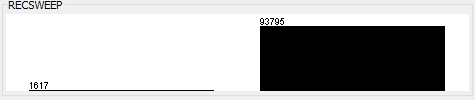
\includegraphics{./images/expl_rep/Cattura-00-03}
%\end{figure}
%\begin{figure}[!ht]
%	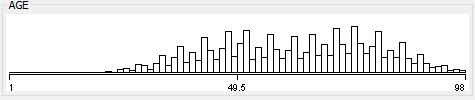
\includegraphics{./images/expl_rep/Cattura-00-04}
%\end{figure}
%\begin{figure}[!ht]
%	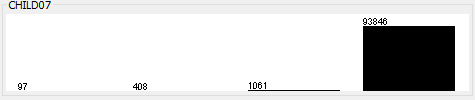
\includegraphics{./images/expl_rep/Cattura-00-05}
%\end{figure}
%\begin{figure}[!ht]
%	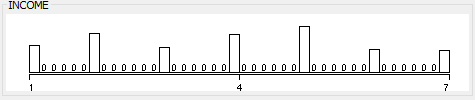
\includegraphics{./images/expl_rep/Cattura-00-06}
%\end{figure}
%\begin{figure}[!ht]
%	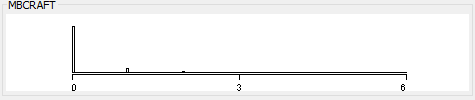
\includegraphics{./images/expl_rep/Cattura-00-07}
%\end{figure}
%\begin{figure}[!ht]
%	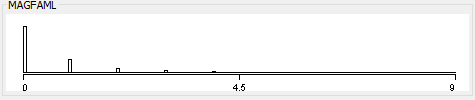
\includegraphics{./images/expl_rep/Cattura-00-08}
%\end{figure}
%\begin{figure}[!ht]
%	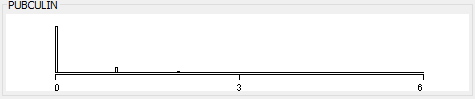
\includegraphics{./images/expl_rep/Cattura-00-09}
%\end{figure}
%\begin{figure}[!ht]
%	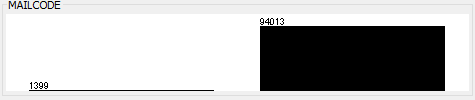
\includegraphics{./images/expl_rep/Cattura-01-01}
%\end{figure}
%\begin{figure}[!ht]
%	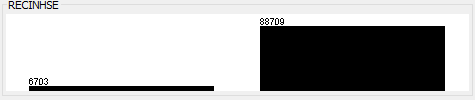
\includegraphics{./images/expl_rep/Cattura-01-02}
%\end{figure}
%\begin{figure}[!ht]
%	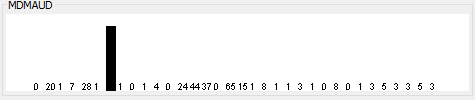
\includegraphics{./images/expl_rep/Cattura-01-03}
%\end{figure}
%\begin{figure}[!ht]
%	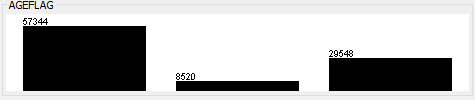
\includegraphics{./images/expl_rep/Cattura-01-04}
%\end{figure}
%\begin{figure}[!ht]
%	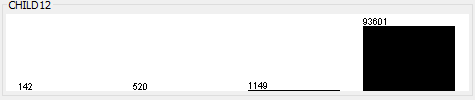
\includegraphics{./images/expl_rep/Cattura-01-05}
%\end{figure}
%\begin{figure}[!ht]
%	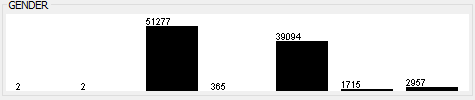
\includegraphics{./images/expl_rep/Cattura-01-06}
%\end{figure}
%\begin{figure}[!ht]
%	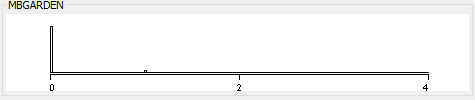
\includegraphics{./images/expl_rep/Cattura-01-07}
%\end{figure}
%\begin{figure}[!ht]
%	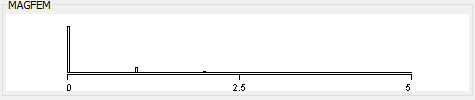
\includegraphics{./images/expl_rep/Cattura-01-08}
%\end{figure}
%\begin{figure}[!ht]
%	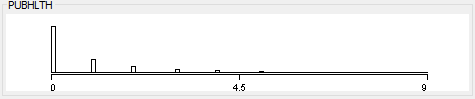
\includegraphics{./images/expl_rep/Cattura-01-09}
%\end{figure}
%\begin{figure}[!ht]
%	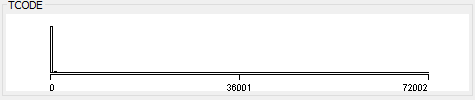
\includegraphics{./images/expl_rep/Cattura-02-00}
%\end{figure}
%\begin{figure}[!ht]
%	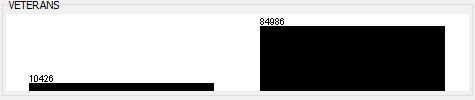
\includegraphics{./images/expl_rep/Cattura2-00-04}
%\end{figure}
	\clearpage
	\chapter{Data Preparation}
\label{ch:datprep}
In questo capitolo verrà valutato come trattare al meglio i dati a disposizione per ragioni di efficienza.

\section{Selezione dei dati}
I dati saranno selezionati principalmente secondo due criteri:
\begin{itemize}
	\item Limitatezza delle risorse (tempo e strumenti di calcolo)
	\item Numero di istanze e di attributi del dataset
\end{itemize}


\section{Sampling}
\label{sec:sampling}
%BEGIN_FOLD
%Il dataset è composto da 95412 istanze, con 90569 esempi negativi e i restanti 4843 esempi positivi, quindi fortmenete sbilanciato; visto l'ingente numero e per l'obsolescenza nota della macchina di lavoro,\ si è deciso di campionare il dataset con l'algoritmo \textbf{Resample} per ottenerne uno più piccolo e più facilmente gestibile, pari al 10\% di quello originario, in più con un bias per rendere uniformi il numero di istanze positive e negative: il nuovo dataset è formato da 9541 istanze, con 4775 istanze negative e 4766 istanze positive, per via dell'uniformità.
%
%\begin{figure}[h!]
%%\begin{subfloat}
%  \begin{subfigure}{.5\textwidth}
%  \centering
%  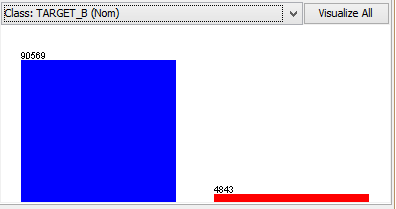
\includegraphics[width=.8\linewidth]{./images/full_unbiased}
%  \caption{Prima: integro e sbilanciato}
%  \label{fig:sfig1}
%  \end{subfigure}
%%\end{subfloat}  
%%\begin{subfloat}
%  \begin{subfigure}{.5\textwidth}
%  \centering
%  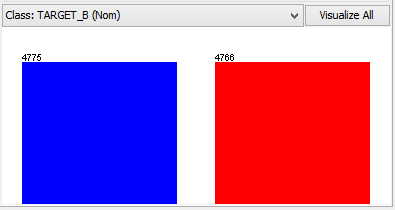
\includegraphics[width=.8\linewidth]{./images/resampled_biased}
%  \caption{Dopo: campionato e bilanciato}
%  \label{fig:sfig2}
%  \end{subfigure}
%%\end{subfloat}  
%  \caption{Versioni del dataset}	
%  \label{fig:fig}
%\end{figure}
%END_FOLD
Il dataset è composto da 95412 istanze, con 90569 esempi negativi e i restanti 4843 esempi positivi, quindi fortmenete sbilanciato. Per superare questo problema si sono svolte le seguenti fasi:
\begin{itemize}
	\item Creazione di nuove istanze per mezzo dell'algoritmo \textit{SMOTE}\cite{Chawla02smote:synthetic}, descritto nella sezione \ref{sec:construct}. Sono stati raddoppiati gli esempi positivi, passando da 4843 a 9686.
	\item Generazione di un sottoinsieme random di istanze grazie all'algoritmo \textit{SpreadSubsample}, che permette di selezionare istanze di classe di maggioranza in maniera casuale. Sono state selezionate 11623 istanze negative rispetto alle 90569 iniziali.
	\item Randomizzazione delle istanze per evitare \textit{overfitting} visto che SMOTE salva le nuove istanze della classe di minoranza in coda al file ARFF.
\end{itemize}

\begin{figure}[htbp!]
	%\begin{subfloat}
	\begin{subfigure}{.5\textwidth}
		\centering
		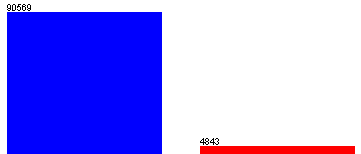
\includegraphics[width=.8\linewidth]{./images/full_unbiased2}
		\caption{Originale}
		\label{fig:unbiased}
	\end{subfigure}
	%\end{subfloat}  
	%\begin{subfloat}
	\begin{subfigure}{.5\textwidth}
		\centering
		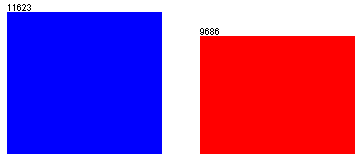
\includegraphics[width=.8\linewidth]{./images/subsampled}
		\caption{Ricampionato}
		\label{fig:sampled}
	\end{subfigure}
	%\end{subfloat}  
	\caption{Versioni del dataset}	
	\label{fig:dataset}
\end{figure}

\pagebreak

\section{Feature selection}
\label{sec:featsel}
%BEGIN_FOLD
%La feature selection ha riguardato la selezione di un sottoinsieme dei 480 attributi, un numero decisamente alto che potrebbe non apportare alcun beneficio ed anzi, potrebbe far incappare nella maledizione della dimensionalità. L'algoritmo utilizzato è l'\textbf{InfoGainAttributeEval} che, come suggerisce il nome, sfrutta la nozione di \emph{Information Gain}, cioè viene scelta la feature che apporti contenuto informativo maggiore rispetto ad un'altra. Presa in considerazione una feature X, l'\emph{Information Gain} IG(X) è definita come la differenza tra una funzione di incertezza a priori, $ \sum_i U(P(c_i)) $, e una funzione di incertezza a posteriori, data X, dove $ U $ è la funzione di incertezza e $ P(c_i) $ rappresenta la probabilità delle classi:
%
%$$ IG(X)=\sum_i U(P(c_i))-E \Big[ \sum_i(P(c_i|X)) \Big] $$
%
%Se $ U(x)=-x\log(x) $, allora $ \sum_i U(P(c_i)) $ è un misura di \textbf{entropia}. \\
%
%La quantità con cui l'entropia decresce rispecchia l'informazione aggiuntiva ottenuta dalla classe dell'attributo.
%Ad ogni attributo è assegnato un punteggio basato sull'information gain tra se stesso e l'attributo target.
%Alla fine dell'elaborazione, gli attributi rimasti sono 220:
%\begin{multicols}{5}
%	\begin{verbatim}
% 		ZIP
% 		DOB
% 		OSOURCE
% 		RFA_4
% 		RFA_3
% 		RFA_6
% 		RFA_9
% 		RFA_2
% 		RFA_8
% 		RFA_16
% 		NEXTDATE
% 		RFA_12
% 		RFA_11
% 		RFA_7
% 		RFA_5
% 		RFA_2F
% 		RFA_22
% 		MAXRDATE
% 		FISTDATE
% 		RFA_19
% 		RFA_17
% 		RFA_18
% 		RFA_14
% 		LASTGIFT
% 		MINRDATE
% 		RFA_21
% 		RFA_2A
% 		RFA_13
% 		RFA_24
% 		RFA_10
% 		LASTDATE
% 		RFA_20
% 		RFA_23
% 		MAXRAMNT
% 		AVGGIFT
% 		RAMNT_8
% 		RAMNT_14
% 		CARDGIFT
% 		PEPSTRFL
% 		MINRAMNT
% 		NGIFTALL
% 		RFA_15
% 		RAMNT_12
% 		STATE
% 		CLUSTER
% 		ODATEDW
% 		NUMPRM12
% 		RAMNT_16
% 		CARDPM12
% 		RAMNT_9
% 		CONTROLN
% 		RAMNT_13
% 		RDATE_14
% 		RAMNT_10
% 		RAMNT_19
% 		RDATE_8
% 		RAMNT_24
% 		CARDPROM
% 		NUMPROM
% 		RAMNT_11
% 		ETHC3
% 		RAMNT_18
% 		RDATE_18
% 		DOMAIN
% 		RAMNT_22
% 		RECP3
% 		RAMNT_15
% 		DMA
% 		RAMNT_7
% 		AGE905
% 		RAMNT_20
% 		POBC2
% 		EC7
% 		RDATE_3
% 		NUMCHLD
% 		RDATE_15
% 		IC15
% 		RAMNT_23
% 		HHD7
% 		EC2
% 		RAMNTALL
% 		HV2
% 		GEOCODE
% 		HVP5
% 		RDATE_19
% 		HV1
% 		HHD9
% 		HHN2
% 		ADATE_7
% 		IC4
% 		VOC2
% 		HHAS4
% 		HVP4
% 		RP1
% 		ADATE_4
% 		HHAS3
% 		RDATE_16
% 		EC1
% 		HVP3
% 		RAMNT_17
% 		HC21
% 		ETH3
% 		RDATE_22
% 		ETHC4
% 		TIMELAG
% 		HC6
% 		HVP2
% 		RDATE_20
% 		RDATE_21
% 		HC2
% 		MARR1
% 		RP3
% 		RDATE_11
% 		TPE4
% 		EC3
% 		RP4
% 		HHAS2
% 		SOLP3
% 		ETH1
% 		VOC1
% 		AGEC6
% 		RP2
% 		RDATE_24
% 		LFC10
% 		RAMNT_3
% 		OCC6
% 		RDATE_4
% 		ETHC5
% 		EC5
% 		AGE906
% 		RAMNT_21
% 		IC10
% 		MDMAUD
% 		RDATE_9
% 		LSC3
% 		RAMNT_4
% 		HHD3
% 		RDATE_6
% 		ETH4
% 		AGE902
% 		ANC2
% 		LSC4
% 		ANC3
% 		HV4
% 		EIC1
% 		OEDC4
% 		TPE12
% 		RDATE_17
% 		MAXADATE
% 		HHD4
% 		HHD1
% 		TCODE
% 		ADATE_8
% 		RDATE_13
% 		RECINHSE
% 		RDATE_7
% 		HOMEOWNR
% 		SOLIH
% 		ADATE_2
% 		AFC3
% 		INCOME
% 		CHILD18
% 		RDATE_23
% 		ADATE_18
% 		CHILD03
% 		RDATE_12
% 		MDMAUD_R
% 		WEALTH2
% 		CHILD12
% 		ADATE_3
% 		DATASRCE
% 		ADATE_12
% 		LIFESRC
% 		ADATE_6
% 		WEALTH1
% 		ADATE_11
% 		WALKER
% 		MDMAUD_F
% 		MDMAUD_A
% 		MAILCODE
% 		GENDER
% 		ADATE_10
% 		RDATE_5
% 		PETS
% 		RDATE_10
% 		NOEXCH
% 		GARDENIN
% 		ADATE_9
% 		PHOTO
% 		GEOCODE2
% 		CRAFTS
% 		ADATE_19
% 		ADATE_23
% 		CARDS
% 		BOATS
% 		ADATE_22
% 		ADATE_16
% 		ADATE_17
% 		CHILD07
% 		MAJOR
% 		ADATE_24
% 		AGEFLAG
% 		ADATE_13
% 		ADATE_14
% 		PVASTATE
% 		CATLG
% 		CDPLAY
% 		BIBLE
% 		KIDSTUFF
% 		HOMEE
% 		ADATE_21
% 		COLLECT1
% 		RECSWEEP
% 		STEREO
% 		RECPGVG
% 		FISHER
% 		PCOWNERS
% 		PLATES
% 		VETERANS
% 		TARGET_B
%LSC4
%HHD1
%HHD4
%ADATE_2
%ADATE_3
%RDATE_3
%RDATE_5
%SOLP3
%RAMNT_4
%ZIP
%RAMNT_3
%RDATE_4
%ADATE_6
%ANC2
%MDMAUD
%HHAS4
%RDATE_6
%MAXADATE
%RAMNT_20
%CONTROLN
%AFC3
%RAMNT_8
%ADATE_4
%ETHC4
%RAMNT_14
%CARDPM12
%ETH3
%RECP3
%MDMAUD_R
%DOB
%RAMNT_7
%LASTGIFT
%MAXRAMNT
%RAMNT_10
%EIC1
%OCC6
%HHD7
%RFA_2F
%RAMNT_9
%RAMNT_12
%RAMNT_13
%NOEXCH
%PEPSTRFL
%MDMAUD_A
%OSOURCE
%NGIFTALL
%RAMNT_23
%RFA_2A
%MDMAUD_F
%RAMNT_11
%AVGGIFT
%RAMNT_17
%RDATE_15
%RAMNT_18
%RAMNT_21
%RAMNT_19
%HHD9
%RAMNT_15
%RAMNT_16
%CARDPROM
%ETHC5
%RFA_2
%OEDC4
%RFA_4
%ADATE_7
%RFA_3
%CHILD03
%HHAS3
%CARDGIFT
%RDATE_14
%RAMNT_24
%MINRAMNT
%RDATE_19
%RDATE_8
%TPE4
%RFA_6
%RDATE_20
%RFA_5
%NUMPRM12
%RDATE_7
%RP1
%RFA_9
%RAMNT_22
%NUMPROM
%ADATE_23
%RFA_23
%EC7
%RAMNTALL
%RDATE_21
%RDATE_18
%RFA_8
%RFA_16
%LASTDATE
%RDATE_9
%RFA_20
%RFA_13
%RFA_12
%RFA_22
%RFA_11
%RFA_7
%VOC2
%RFA_21
%RFA_17
%RFA_19
%NUMCHLD
%MAILCODE
%CHILD18
%MAXRDATE
%CHILD12
%RFA_24
%RFA_14
%RFA_10
%RFA_18
%ETH1
%NEXTDATE
%ADATE_14
%RFA_15
%FISTDATE
%MAJOR
%ADATE_24
%ADATE_8
%DMA
%RDATE_17
%MINRDATE
%RDATE_11
%IC15
%HV2
%POBC2
%RDATE_23
%RDATE_22
%RECINHSE
%SOLIH
%LFC10
%RDATE_13
%HV1
%EC2
%MARR1
%RDATE_16
%ETHC3
%HVP3
%HVP4
%IC4
%HVP5
%HC21
%HHD3
%TPE12
%HHN2
%VOC1
%ODATEDW
%RDATE_24
%HC6
%EC3
%GEOCODE
%CARDS
%LSC3
%HC2
%AGE905
%EC1
%ETH4
%TIMELAG
%STATE
%RP4
%HVP2
%IC10
%RP3
%ADATE_19
%EC5
%AGE906
%AGEC6
%RP2
%HHAS2
%CLUSTER
%ADATE_13
%AGE902
%ADATE_10
%ANC3
%HV4
%TCODE
%INCOME
%BOATS
%ADATE_9
%RDATE_10
%ADATE_16
%DOMAIN
%CHILD07
%ADATE_18
%RDATE_12
%PHOTO
%WALKER
%HOMEOWNR
%PETS
%CRAFTS
%GARDENIN
%ADATE_12
%PVASTATE
%ADATE_11
%RECPGVG
%ADATE_17
%ADATE_22
%DATASRCE
%LIFESRC
%GENDER
%WEALTH2
%HOMEE
%WEALTH1
%KIDSTUFF
%GEOCODE2
%CATLG
%RECSWEEP
%BIBLE
%AGEFLAG
%CDPLAY
%ADATE_21
%COLLECT1
%PLATES
%STEREO
%FISHER
%PCOWNERS
%VETERANS
%TARGET_B
%	\end{verbatim}
%\end{multicols}
%END_FOLD
Come algoritmo di feature selection si è scelto il \emph{CfsSubsetEval}, che valuta il miglior subset degli attributi considerando la singola correlazione di ognuno con l'attributo di classe. Si sceglierà il subset con la più alta correlazione con l'attributo target, ma allo stesso tempo con una bassa correlazione con gli altri attributi. La ricerca nello spazio del subset degli attributi viene realizzata attraverso la strategia \textit{best first}, cercando di avvicinarsi ad un risultato ottimale in maniera \textit{greedy}, tagliando lo spazio di ricerca con la tecnica del \textit{backtracking}\cite{Hall1998}.
L'algoritmo può operare in tre modi:
\begin{itemize}
	\item Partire da un insieme di feature vuoto e incrementarlo, aggiungendo le più predittive.
	\item Partire dall'insieme contenente tutte le feature e ridurlo, eliminando quelle meno predittive.
	\item Partire da un qualsiasi punto e muoversi in entrambe le direzioni aggiungendo e rimuovendo feature.
\end{itemize}

Le feature rimanenti per \tb{} sono le seguenti:
\begin{multicols}{3}
	\begin{verbatim}
		HIT
		MALEMILI
		STATEGOV
		ETH3
		ETH6
		ETH7
		ETH8
		ETH10
		ETH14
		ETH16
		DW3
		DW8
		DW9
		HHD8
		ETHC6
		HUR1
		IC13
		TPE4
		TPE6
		TPE7
		TPE8
		PEC1
		OCC6
		OCC7
		EIC1
		EIC2
		EIC3
		EIC6
		EIC7
		EIC10
		EIC11
		EIC12
		EIC13
		OEDC5
		OEDC7
		SEC1
		SEC3
		AFC1
		AFC6
		ANC1
		ANC3
		ANC6
		ANC8
		ANC9
		ANC10
		ANC12
		ANC13
		ANC14
		ANC15
		HC3
		HC10
		HC14
		MHUC2
		AC2
		MAXADATE
		CARDPM12
		MINRAMNT
		RFA_2F
		RFA_2A
	\end{verbatim}
\end{multicols}

\section{Pulizia dei dati}
In questa fase sono stati trattate le variabili che presentano rumore e \emph{missing values}.

Il rumore si è avuto sui campi di tipo data che nel dataset originario avevano il formato "aaMM"; per risolvere i problemi sono stati rimossi gli \textit{outlier} che non rispettavano alcun formato di data conosciuto in quanto erano delle semplici cifre.

Un altro campo che conteneva degli outlier era \textit{GENDER}: tali valori sono stati rimpiazzati dalla moda.

Per quanto riguarda i missing value, sono stati rimossi gli attributi che ne contavano più del 70\%. Gli attributi rimossi sono 53.

Per gli altri attributi con il numero di missing value minore del 70\%, sono stati rimpiazzati quelli numerici dalla media dei presenti, mentre quelli categorici dalla moda.

\section{Costruzione di nuovi dati}
\label{sec:construct}
In questa fase sono state trattate due situazioni, la conversione delle date e l'incremento di istanze per mitigare lo sbilanciamento iniziale.

All'atto del caricamento del dataset in Weka, i campi di tipo data non erano trattati come tali ma come dati numerici, quindi sono stati convertiti in tipo \textit{Date}, gestito da Weka, e poi ne è stato cambiato il formato, da "aaMM" a "aaaa-MM", per una migliore gestione.

Per via della limitato numero di istanze della classe di minoranza, ne sono state generate di nuove utilizzando l'algoritmo \textit{SMOTE}.
\subsection{SMOTE}
\label{SMOTE}
SMOTE permette di ricampionare il dataset in maniera supervisionata utilizzando la \textbf{S}ynthetic \textbf{M}inority \textbf{O}versampling \textbf{TE}chnique\cite{Chawla02smote:synthetic}. Questa tecnica combina l'\emph{Information Oversampling} della classe minorante, con la \emph{Random Undersampling} della maggiorante. Di seguito l'algoritmo per effettuare il sovracampionamento della classe minorante.

\begin{algorithm}[!htb]
	\caption{\emph{SMOTE’s Informed Oversampling Procedure}}
	\begin{algorithmic}[1]
		\ForAll{Campione di minoranza}
				\State Trova i suoi $k$-viciniori di minoranza
				\State Selezionane $j$ in modo casuale
				\State Genera campioni sintetici in modo casuale unendo il campione di minoranza e i suoi $j$ viciniori ($j$ dipende dal grado di oversampling desiderato)
		\EndFor
	\end{algorithmic}
\end{algorithm}

%\pagebreak

Al termine dell'operazione le istanze di minoranza sono passate da 4843 a 9686. Successivamente verrà applicato \textit{SpreadSunsample} per ridurre il divario tra il numero delle istanze, come visto nella figura \ref{fig:sampled}.

\begin{figure}[!htb]
	\centering
	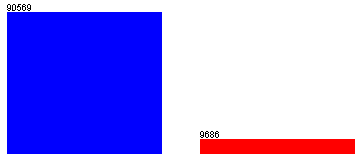
\includegraphics[width=.6\linewidth]{./images/smoted}
	\caption{Dataset dopo SMOTE, non ancora ricampionato}
\end{figure}


\section{Integrazione dei dati}
Non è stata compiuta alcuna operazione di integrazione o fusione con sorgenti dati di terze parti.

\section{Formato dei dati}
Il formato del dataset era in orgine il \textbf{Comma Separated Value} (CSV), ma per renderlo più maneggevole è stato convertito in \textbf{Attribute-Relation File Format} (ARFF).
	\clearpage
    \chapter{Modeling}
\label{ch:model}
Ai fini della classificazione, si è scelto di usare l'algoritmo \textbf{RIPPER}\cite{Cohen95fasteffective}, in particolare nella versione implementata da Weka, \textbf{JRip}\cite{Witten:2011:DMP:1972514}.

\section{Tecnica di modeling}
RIPPER (\textbf{R}epeated \textbf{I}ncremental \textbf{P}runing to \textbf{P}roduce \textbf{E}rror \textbf{R}eduction) è un algoritmo di induzione di regole proposto da \verb|William W. Cohen| nel 1995. Esso si è dimostrato competitivo con C4.5Rules rispetto ai tassi di errore, scala in maniera lineare con il numero di esempi di training e può elaborare in maniera efficiente dataset rumorosi che contengono centinaia di migliaia di esempi. RIPPER si basa su IREP (\textbf{I}ncremental \textbf{R}educed \textbf{E}rror \textbf{P}runing))\cite{Furnkranz94incrementalreduced}, di cui si discuterà nei prossimi paragrafi.
\section{Rappresentazione del modello}
Molte delle tecniche usate nei moderni sistemi di apprendimento di regole  sono stati adattate dall'apprendimento degli alberi di decisione. La maggior parte dei sistemi di apprendimento di alberi di decisione usa una strategia di appredimento \textit{overfit-and-simplify} (sovradatta-e-semplifica) per gestire dati rumorosi: viene generata un'ipotesi prima facendo crescere un albero complesso che "overfitta" i dati, e poi si semplifica o pota tale albero (un'operazione di \textit{pruning}). Una tecnica di pruning efficace è \textit{reduced error pruning} (\textit{REP}). Essa può essere facilmente adattata ai sistemi di apprendimento di regole\cite{Pagallo1990}\cite{Brunk91aninvestigation}.

In REP per le regole, il training set viene diviso in \textit{growing set} e \textit{pruning set}. All'inizio, viene creato un \textit{rule set} di partenza che overfitta il growing set, usando qualche metodo euristico. Questo rule set spropositato viene poi semplificato ripetutamente applicando qualche operatore di pruning. Ad ogni fase di semplificatione, l'operatore di pruning scelto è quello che produce la più grande riduzione di errore sul pruning set. La semplificazione finisce quando il tasso di errore non si riduce ulteriormente applicando gli operatori di pruning.

REP per le regole di solito migliora davvero la perfomance di generalizzazione sui dati rumorosi\cite{Pagallo1990}\cite{Brunk91aninvestigation}\cite{Weiss91reducedcomplexity}\cite{Furnkranz94incrementalreduced}; tuttavia è computazionalmente costoso per grandi dataset\cite{Cohen93efficientpruning}.

In risposta all'inefficienza di REP, Fürnkranz e Widmer [1994] proposero un algoritmo di apprendimento chiamato \textit{incremental reduced error pruning} (\textit{IREP})\cite{Furnkranz94incrementalreduced}.

\subsection*{Incremental Reduced Error Pruning}
L'idea di usare un pruning set separato per la potatura è REP. La variante che pota una regola subito dopo averla "fatta crescere" si chiama \textit{incremental reduced error pruning} (IREP)\cite{2Witten:2011:DMP:1972514}. Quest'ultima integra saldamente REP con un algoritmo di apprendimento di regole \textit{separate-and-conquer}. L'algoritmo \ref{alg:irep} ne presenta una versione a due classi. Come ogni algoritmo separate-and-conquer standard, IREP costruisce un ruleset in maniera \textit{greedy}, una regola alla volta. Dopo averne trovata una, tutti gli esempi coperti da quella regola (sia positivi che negativi) sono cancellati. Questo processo si ripete finché non ci sono più esempi positivi, o finché la regola trovata da IREP non presenta un grande tasso di errore, cosa inaccettabile.

Per costruire una regola, IREP usa la seguente strategia. Prima, gli esempi non coperti sono partizionati a caso in due sottoinsiemi, un growing e un pruning set. Nell'implementazione di Cohen, il growing set contiene 2/3 degli esempi.

Poi, una regola viene "fatta crescere". L'implementazione di Cohen di $GrowRule$ è una versione proposizionale di FOIL (First Order Inductive Learner), dove i letterali non si servono di predicati ma di uguaglianze (per valori discreti) e confronti numerici (per valori continui)\cite{Russell:2003:AIM:773294}. Esso inizia con una congiunzione vuota di condizioni (la regola vuota) e considera di aggiungere a questa qualsiasi condizione nella forma $A_d=v$, $A_c \leq \theta$ oppure $A_c \geq \theta$ dove $A_d$ è un attributo discreto e $v$ è un valore che può assumere, mentre $A_c$ è un attributo continuo e $\theta$ è un valore soglia. $GrowRule$ aggiunge ripetutamente la condizione che massimizza un'euristica di \emph{information gain}, nello specifico quella di FOIL, finché la regola non copre più esempi negativi nel growing set.

Siano $R_0$ e $R_1$ due regole, la seconda ottenuta dall'aggiunta di una condizione nel corpo della prima. L'information gain viene così calcolato:

$$
Gain(R_0,R_1) = t \times \left(\log{\dfrac{p_1}{p_1 + n_1}} - \log{\dfrac{p_0}{p_0 + n_0}}\right)
$$

dove $t$ riguarda gli esempi positivi coperti da $R_0$ che soddisfano anche $R_1$ dopo aver aggiunto una condizione, $p_0$ (rispettivamente $p_1$) sono gli esempi positivi coperti da $R_0$ (rispettivamente $R_1$) e  $n_0$ (rispettivamente $n_1$) sono gli esempi negativi coperti da $R_0$ (rispettivamente $R_1$).

L'idea alla base è che l'informazione totale che si guadagna è dato dal numero di tuple che soddisfano la nuova condizione moltiplicato l'informazione guadagnata in merito a ciascuna\cite{Quinlan1990}.

Dopo aver espanso una regola, essa viene immediatamente potata. Per prunarla, l'implementazione di Cohen cancella qualsiasi sequenza finale di condizioni dalla regola e sceglie l'eliminazione che massimizza la funzione
\begin{equation}
	\label{eq:rulval}
	v(Rule, PrunePos, PruneNeg) \equiv \frac{p + (N - n)}{P + N}
\end{equation}

dove $P$ (rispettivamente $N$) è il numero totale di esempi in $PrunePos$ \linebreak ($PruneNeg$) e $p$ ($n$) è il numero di esempi in $PrunePos$ ($PruneNeg$) coperti da $Rule$. Questo processo è ripetuto finché nessun altra cancellazione migliora il valore di $v$.

L'algoritmo IREP descritto sopra è per i problemi di apprendimento a due classi. L'implementazione di Cohen gestisce classi multiple, come spiegato di seguito:
\begin{enumerate}
	\item Le classi vengono ordinate secondo la prevalenza, cioè l'ordine è $C_1,...,C_k$ dove $C_1$ è la classe di minoranza e $C_k$ è la classe di maggioranza.
	\item Viene trovata una regola che separi $C_1$ dal resto delle classi; questo viene fatto con una singola chiamata ad IREP dove $PosData$ contiene gli esempi di classe $C_1$ e $NegData$ contiene gli esempi di classi $C_2,C_3,...,C_k$.
	\item Tutte le istanze coperte dal ruleset appena addestrato sono rimosse dal dataset e IREP si appresta a separare $C_2$ dalle classi $C_3,...,C_k$.
	\item Si ripete finché rimane la sola classe $C_k$. Quest'ultima verrà usata come classe di default.
\end{enumerate}

L'implementazione di Cohen differisce da quella di Fürnkranz e Widmer sotto molti aspetti. Quando le regole vengono potate, la nuova implementazione permette di cancellare qualsiasi sequenza finale di condizioni, mentre l'implementazione di Fürnkranz e Widmer permette solo la cancellazione di una singola condizione finale. L'algoritmo rivisitato permette anche di fermare l'aggiunta di regole al ruleset quando la regola appresa ha un tasso di errore superiore al 50\%, mentre quello di Fürnkranz e Widmer la ferma quando l'accuratezza della regola è minore 
dell'accuratezza della regola vuota.

\begin{algorithm}[!htbp]
	\caption{IREP($Pos, Neg$)}
	\label{alg:irep}
	\begin{algorithmic}[1]
		\State $Ruleset \gets \emptyset$
		
		\While{Pos $\neq \emptyset$}
		\State dividi $(Pos, Neg)$ in $(GrowPos, GrowNeg)$ e $(PrunePos, PrunNeg)$
		\State $Rule \gets GrowRule(GrowPos, GrowNeg)$
		\State $Rule \gets PruneRule(Rule, PrunePos, PruneNeg)$
		
		\If{il tasso di errore su $(PrunePos, PrunNeg) > 50\%$}
		\State \Return $Ruleset$
		\Else
		%\State $Ruleset \gets Ruleset \cup \{Rule\}$
		\State aggiungi $Rule$ a $Ruleset$
		\State rimuovi gli esempi coperti da $Rule$ da $(Pos, Neg)$
		\EndIf
		\EndWhile
		
		\State \Return $Ruleset$
	\end{algorithmic}
\end{algorithm}

\pagebreak

\subsection*{Miglioramenti ad IREP}
Sono state implementate tre modifiche ad IREP: una metrica alternativa per determinare il valore delle regole nella fase di potatura; una nuova euristica per dedidere quando fermare l'aggiunta di regole al ruleset; un successivo passaggio di "ottimizzazione" del ruleset per tentare di avvicinarsi di più al REP convenzionale (cioè, non incrementale).

\subsubsection*{Metrica per il valore delle regole}
Il fallimento occasionale di IREP a convergere al crescere del numero degli esempi può essere facilmente fatto risalire alla metrica usata per guidare la potatura (ossia la \eqref{eq:rulval}). Le scelte intraprese nella definizione di tale metrica non sono intuitive; per esempio (assumendo che $P$ e $N$ siano fissati) la metrica preferisce una regola $R_1$ che copre $p_1 = 2000$ esempi positivi e $n_1 = 1000$ esempi negativi rispetto ad una regola $R_2$ che copre $p_2 = 1000$ esempi positivi e $n_2 = 1$ esempio negativo; si noti comunque che $R_2$ è altamente predittiva, al contrario di $R_1$. Quindi si è deciso di sostituire la metrica di IREP con $$v^*(Rule, PrunePos, PruneNeg) \equiv \frac{p - n}{p + n}$$ che sembra avere un comportamento più intuitivo e soddisfacente.

\subsubsection*{Condizione di stop}
L'implementazione di IREP di Cohen si ferma in maniera greedy aggiungendo regole al ruleset quando l'ultima regola costruita ha un tasso d'errore maggiore del 50\% sui dati di pruning. Questa euristica, spesso, si ferma troppo presto con campioni di dimensioni moderate; questo è vero soprattutto quando si apprende un concetto con regole a bassa copertura (pochi esempi coperti).

La soluzione a questo problema è la seguente. Dopo l'aggiunta di ogni regola, viene calcolata la \textit{description-length} totale del ruleset e degli esempi. La nuova versione di IREP ferma l'aggiunta di regole quando questa description-length è maggiore di $d$ bit rispetto alla più piccola description-length ottenuta sinora, o quando non ci sono più esempi positivi. Nell'implementazione si è usato $d = 64$. Il ruleset viene poi semplificato esaminando ogni regola a turno (cominciando dall'ultima) e cancellando regole così da ridurre la description-length totale. 

Il principio \emph{MDL} (Minimum Description Length) può essere meglio espresso immaginando un modello di comunicazione in cui un mittente trasmette ad un ricevente una descrizione che consiste in una teoria $T$ e i dati $D$ da cui essa è derivata\cite{Quinlan:1989:IDT:70758.70761}.

Il metodo usato per la codifica è lo stesso usato in \emph{C4.5rules}\cite{Quinlan95mdland}. Esso parte da un \emph{bias} in cui il numero di falsi positivi e falsi negativi sia lo stesso e si procede come segue: i messaggi da inviare si presentano con probabilità $p_j$, e servono $-\log(p_j)$ bit (in base 2) per costrurli: più un messaggio è frequente, meno bit saranno necessari per rappresentarlo. Si inviano i dati codificati, poi anziché inviare i messaggi di errore per tutti i dati, il mittente prima trasmette gli errori $e$ nei $C$ casi coperti dalla teoria e poi negli $U$ casi non coperti. Sotto l'assunzione che i falsi positivi $fp$ e i falsi negativi $fn$ siano bilanciati, la probabilità di errore nei casi coperti è $e/2C$ e questa probabilità è usata per codificare i messaggi di errore per i casi coperti. Una volta che i falsi positivi sono stati identificati, il destinatario può calcolare il vero numero dei falsi negativi come $e-fp$, quindi la probabilità di errore oer i casi non coperti è $fn/U$. Il costo totale quindi diventa:

\begin{align*}
	&\log(|D| + 1) \\
	&+ fp \times (-\log(\dfrac{e}{2C})) \\
	&+ (C - fp) \times (-\log(1 - \-\dfrac{e}{2C})) \\
	&+ fn \times (-\log(\dfrac{fn}{U})) \\
	&+ (U - fn) \times (-\log(1 - \dfrac{fn}{U})) \\	
\end{align*}


\subsubsection*{Ottimizzazione delle regole}
L'approccio ripetuto \textit{grow-and-simplify} usato in IREP può produrre risultati abbastanzi differenti dal REP convenzionale (non incrementale). Un modo per migliorarlo è elaborare a posteriori le regole prodotte da IREP così da avvicinarsi di più all'effetto del REP convenzionale. Per esempio, si potrebbe ri-potare ogni regola al fine di minimizzare l'errore del ruleset completo.

Il metodo sviluppato per ottimizzare un ruleset $R_1,R_2,...,R_k$ consiste del costruire due regole alternative per ogni $R_i$. La \textit{sostituta} di $R_i$ viene generata espandendo e poi potando $R_i$. La \textit{revisione} di $R_i$ viene generata in maniera analoga, tranne per il fatto che la revisione è espansa in modo greedy aggiungendo condizioni a $R_i$, piuttosto che alla regola vuota. Infine si sceglie tra le tre regole quale includere nella teoria. Questa decisione viene presa in base all'euristica MDL. L'implementazione di questo metodo in IREP avviene in questo modo:
\begin{enumerate}
	\item Viene usato IREP per ottenere un ruleset iniziale.
	\item Esso viene ottimizzato, come descritto sopra.
	\item Vengono aggiunte le regole in modo tale da coprire gli esempi positivi rimanenti.
\end{enumerate}

L'ottimizzazione può essere ripetuta più volte elaborando il ruleset ottenuto dalla passata precedente dell'algoritmo.

IREP, con l'aggiunta del passo di post-ottimizzazione, forma un nuovo algoritmo che è stato chiamato \textbf{RIPPER} (\textbf{R}epeated \textbf{I}ncremental \textbf{P}runing to \textbf{P}roduce \textbf{E}rror \textbf{R}eduction).

L'implementazione in Weka di RIPPER si chiama JRip.

\section{Costruzione del modello}
I parametri per la costruzione del modello con l'algoritmo JRip sono i seguenti:
\begin{center}
	\begin{tabular}{|r|l|}
		\hline
		\textbf{checkErrorRate} & \texttt{True} \\ \hline
		\textbf{debug} & \texttt{False} \\ \hline
		\textbf{doNotCheckCapabilities} & \texttt{False} \\ \hline
		\textbf{folds} & \texttt{3} \\ \hline
		\textbf{minNo} & \texttt{2.0} \\ \hline
		\textbf{optimizations} & \texttt{2} \\ \hline
		\textbf{seed} & \texttt{1} \\ \hline
		\textbf{usePruning} & \texttt{True} \\ \hline
	\end{tabular}
\end{center}

Inoltre, la configurazione del modello ha previsto:
\begin{itemize}
	\item Per il sampling \textbf{SpreadSubsample} e \textbf{SMOTE} (\ref{sec:sampling}).
	\item Per la feature selection l'algoritmo \textbf{CfsSubsetEval} (\ref{sec:featsel}).
\end{itemize}

%\raggedright
\noindent
Il modello costruito da JRip contiene 10 regole:
\begin{verbatimtab}
(RFA_2A = C)		and
(IC13 >= 0.000028)	and
(ANC9 >= 0.000195)	and
(MINRAMNT >= 3.003216)	and
(PEC1 >= 0.000121)	=> TARGET_B=1 (2231.0/5.0)

(RFA_2A = C)		and
(SEC3 >= 2.003965)	and
(MALEMILI >= 0.000547)	and
(MALEMILI <= 0.999097)	=> TARGET_B=1 (901.0/0.0)

(RFA_2A = C)		and
(SEC3 >= 2.000523)	and
(SEC3 <= 2.990595)	=> TARGET_B=1 (630.0/0.0)

(RFA_2A = C)		and
(SEC1 >= 3.015142)	and
(ANC13 <= 0.999471)	and
(ANC13 >= 0.001289)	=> TARGET_B=1 (370.0/0.0)

(RFA_2A = C)		and
(HIT >= 2.0117)		and
(TPE4 >= 1.029922)	and
(ETH16 <= 0.999469)	=> TARGET_B=1 (289.0/18.0)

(RFA_2A = C)		and
(ETH8 >= 0.001684)	and
(ETH8 <= 0.997973)	=> TARGET_B=1 (209.0/0.0)

(RFA_2A = C)		and
(MHUC2 >= 2.000098)	and
(MHUC2 <= 2.999771)	=> TARGET_B=1 (110.0/0.0)

(RFA_2A = C)		and
(MALEMILI >= 0.049379)	and
(ANC10 >= 0.142011)	and
(MINRAMNT <= 2.979151)	and
(ANC13 <= 0.953307)	=> TARGET_B=1 (68.0/5.0)

(RFA_2A = C)		and
(HIT >= 2.247392)	and
(IC13 >= 0.034224)	and
(ANC15 >= 0.031307)	=> TARGET_B=1 (41.0/4.0)

[Empty Rule]		=> TARGET_B=0 (16460.0/4869.0)
\end{verbatimtab}

\subsection{Interpretazione del modello}
Gli attributi presenti nelle regole necessitano di un po' di chiarezza, quindi di seguito vengono descritti:

\begin{center}
\begin{tabularx}{\textwidth}{|c|X|}
	\hline
	\texttt{RFA\_2A} & Codice per l'ammontare della donazione passata: \\ &
		- L = Meno di \$100 (Low Dollar) \\ &
		- C = \$100 - \$499  (Core) \\ &
		- M = \$500 - \$999 (Major) \\ &
		- T = \$1,000+ (Top) \\

 \hline
	
	\texttt{IC13} & Percentuale dei membri del nucleo abitativo con reddito tra \$125,000 e \$149,999\\ \hline
	
	\texttt{ANC9} & Percentuale di ascendenza norvegese\\ \hline
	
	\texttt{MINRAMNT} & Ammontare in dollari dell'ultimo dono spedito\\ \hline
	
	\texttt{PEC1} & Percentuale di lavoro effetuato fuori dallo stato di residenza\\ \hline
	
	\texttt{SEC3} & Percentuale di persone iscritte all'asilo\\ \hline
	
	\texttt{MALEMILI} & Percentuale di maschi attivi in forze militari\\ \hline
	
	\texttt{SEC1} & Percentuale persone iscritte in scuole private\\ \hline
	
	\texttt{ANC13} & Percentuale di ascendenza scozzese\\ \hline
	
	\texttt{HIT} & Numero di volte conosciute in cui il donatore ha risposto a offerte postali diverse da quella dell'organizzazione\\ \hline
	
	\texttt{TPE4} & Percentuale che usano bus/tram\\ \hline
	
	\texttt{ETH16} & Percentuale di altra etnia ispanica\\ \hline
	
	\texttt{ETH8} & Percentuale di cinesi\\ \hline
	
	\texttt{MHUC2} & Mediana dei costi di proprietari di case senza ipoteca mensile, in dollari\\ \hline
	
	\texttt{ANC10} & Percentuale di ascendenza polacca\\ \hline
	
	\texttt{ANC13} & Percentuale di ascendenza scozzese\\ \hline
	
	\texttt{ANC15} & Percentuale di ascendenza ucraina\\ \hline
\end{tabularx}
\end{center}

La teoria mostra chiaramente che la condizione più discriminante è \verb|RFA_2A = C|, presente in tutte le regole, che codifica la quantità di denaro inviata alla fondazione in passato.

Quindi è necessario che il donatore abbia versato, in passato, una somma compresa tra i 100 e 499 dollari. Altre informazioni di carattere economico riguardano il reddito dei membri del nucleo abitativo (\texttt{IC*}) o la mediana dei costi delle case (\texttt{MHUC2}), ignorando eventuali ipoteche e il valore dell'ultimo dono spedito al donatore (\texttt{MINRAMNT}).

Altre considerazioni che si possono fare riguardano le informazioni sulla razza dei donatori e sul loro nucleo famigliare/abitativo, indicate dagli attributi di ascendeza (\texttt{ANC*}) ed etnia (\textsc{ETH*}), oppure sul livello di scolarizzazione (\texttt{SEC*}) o di prestazione di servizi militari (\texttt{MALEMILI}).

\section{Valutazione del modello}
I risultati ottenuti da Weka sono i seguenti:
\begin{mdframed}
\begin{verbatim}
=== Stratified cross-validation ===
=== Summary ===

Correctly Classified Instances       16340               76.6812 %
Incorrectly Classified Instances      4969               23.3188 %
Kappa statistic                          0.5092
Mean absolute error                      0.3265
Root mean squared error                  0.4052
Relative absolute error                 65.8419 %
Root relative squared error             81.3854 %
Coverage of cases (0.95 level)          99.8123 %
Mean rel. region size (0.95 level)      88.8216 %
Total Number of Instances            21309     

=== Detailed Accuracy By Class ===

           TP Rate  FP Rate  Precision  Recall   F-Measure  ROC Area  Class
           0,996    0,508    0,702      0,996    0,823      0,746     0
           0,492    0,004    0,990      0,492    0,657      0,746     1
W. Avg.    0,767    0,279    0,833      0,767    0,748      0,746     

=== Confusion Matrix ===

a     b   <-- classified as
11574   49 |     a = 0
4920  4766 |     b = 1
\end{verbatim}
\end{mdframed}
%\begin{verbatim}
%=== Stratified cross-validation ===
%=== Summary ===
%
%Correctly Classified Instances       16374               76.8408 %
%Incorrectly Classified Instances      4935               23.1592 %
%Kappa statistic                          0.5126
%Mean absolute error                      0.325 
%Root mean squared error                  0.4042
%Relative absolute error                 65.5513 %
%Root relative squared error             81.1661 %
%Coverage of cases (0.95 level)          99.8358 %
%Mean rel. region size (0.95 level)      88.8709 %
%Total Number of Instances            21309     
%
%=== Detailed Accuracy By Class ===
%
%           TP Rate  FP Rate  Precision  Recall   F-Measure  ROC Area  Class
%           0,996    0,505    0,703      0,996    0,824      0,748     0
%           0,495    0,004    0,991      0,495    0,660      0,748     1
%W. Avg.    0,768    0,277    0,834      0,768    0,750      0,748     
%=== Confusion Matrix ===
%
%a      b   <-- classified as
%11580    43 |     a = 0
%4892   4794 |     b = 1
%\end{verbatim}

Il modello fornisce una classificazione corretta al 76,8408\%, contro il 23,1592\% di classificare in modo errato.
    \clearpage
    \chapter{Evaluation}
\label{ch:eval}
In questo capitolo verranno riportati e valutati i risultati ottenuti dall’intero processo KDD.

\section{Valutazione dei risultati}

Il processo KDD terminerà con successo se si riuscirà a costruire un modello che soddisfi il task.
\subsection{KnowledgeFlow}

\begin{figure}[hbtp!]
	\centering
	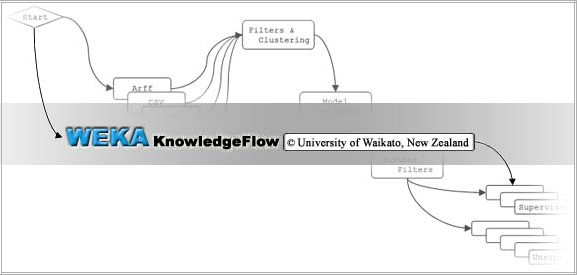
\includegraphics[width=0.6\textwidth]{./images/kf}
  	\caption{Logo di Weka KnowledgeFlow}  
\end{figure}

Per velocizzare le operazioni di confronto tra diverse tecniche di modeling si è scelto di usare lo strumento \textbf{KnowledgeFlow}, fornito sempre da Weka.

In KnowledgeFlow, l'utente può selezionare le componenti di Weka dalla barra degli strumenti, trascinarle su un canvas e collegarle l'una all'altra per formare un flusso per elaborare ed analizzare dati. Sono disponibili molti filtri, classificatori ed altri algoritmi già disponibili nell'Explorer di Weka, insieme ad altri strumenti, tipo la possibilità di salvare i risultati dell'elaborazione su un file, vedere grafici ecc.

Caratteristiche di KnowledgeFlow:
\begin{itemize}
	\item Layout intuitivo per rappresentare il flusso dei dati.
	\item Elaborazione dei dati in modalità batch o incrementale
    \item Elaborazione di più batch o stream in parallelo (ogni flusso ha il suo thread dedicato).
    \item Concatenazione di filtri.
    \item Visualizzazione delle performance dei classificatori al termine dell'elaborazione.
\end{itemize}

\subsection{Configurazioni}
Le configurazioni per la valutazione hanno visto l'utilizzo di due algoritmi, Ripper e C4.5 (rispettivamente JRip e J48 in Weka) al variare di alcuni parametri.

\begin{figure}[!htbp]
	\hspace*{-1.1in}
	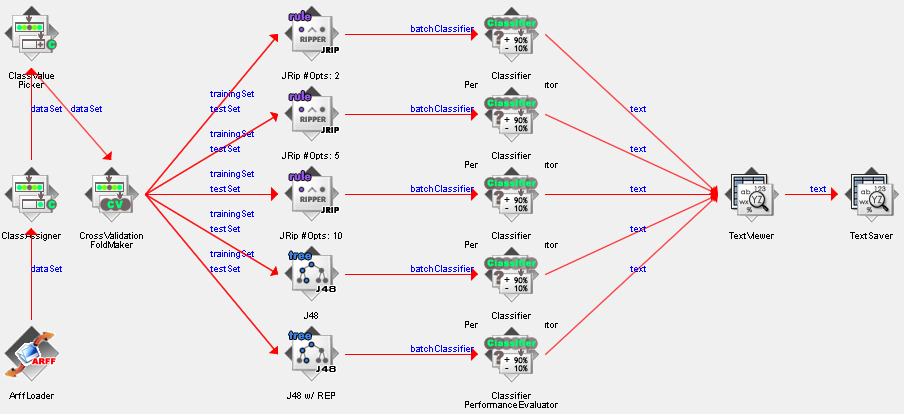
\includegraphics[width=1.4\textwidth]{./images/flow3}
\end{figure}

Nella fattispecie, le configurazioni sono:
\begin{itemize}
	\item JRip con 2 passate successive di ottimizzazione (default).
	\item JRip con 5 passate successive di ottimizzazione.
	\item JRip con 10 passate successive di ottimizzazione.
	\item J48 con pruning di default (\textit{Error-Based Pruning})\cite{Quinlan:1993:CPM:152181}.
	\item J48 con pruning effettuato da REP.
\end{itemize}
%Le varie configurazioni hanno previsto l'utilizzo di 3 tecniche di modeling, \textbf{IB1}, \textbf{Naive Bayes} e \textbf{C4.5} (quest'ultima implementata con l'algortimo J48). Ognuna ha lavorato sul dataset completo con tutti gli attributi iniziali e sulla sua versione ridotta ottenuta dalla feature selection. Inoltre per IB1 sono stati considerati diversi livelli di \emph{neighbours}, ovvero 1, 3 e 5.
%
%Questo è lo schema del workflow senza feature selection:
%
%\begin{figure}[hbtp!]
%	\hspace*{-1.1in}
%	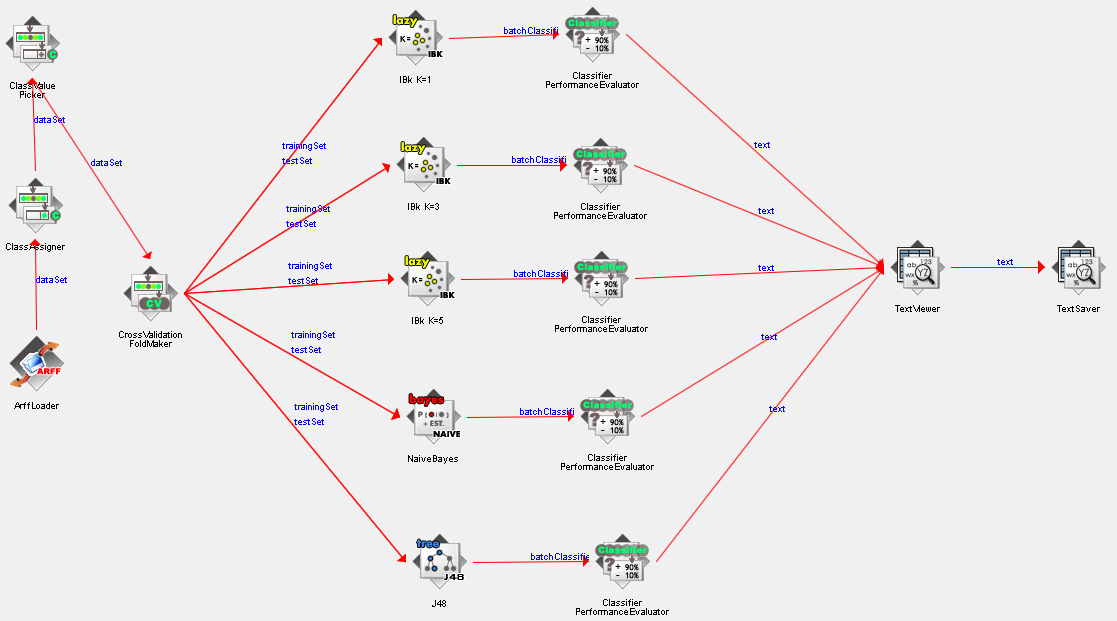
\includegraphics[width=1.4\textwidth]{./images/flow_no_featsel}
%\end{figure}
%
%Questo invece è lo schema con feature selection; l'unica differenza è la presenza della componente di filtraggio "AttributeSelection":
%
%\begin{figure}[hbtp!]
%	\hspace*{-1.1in}
%	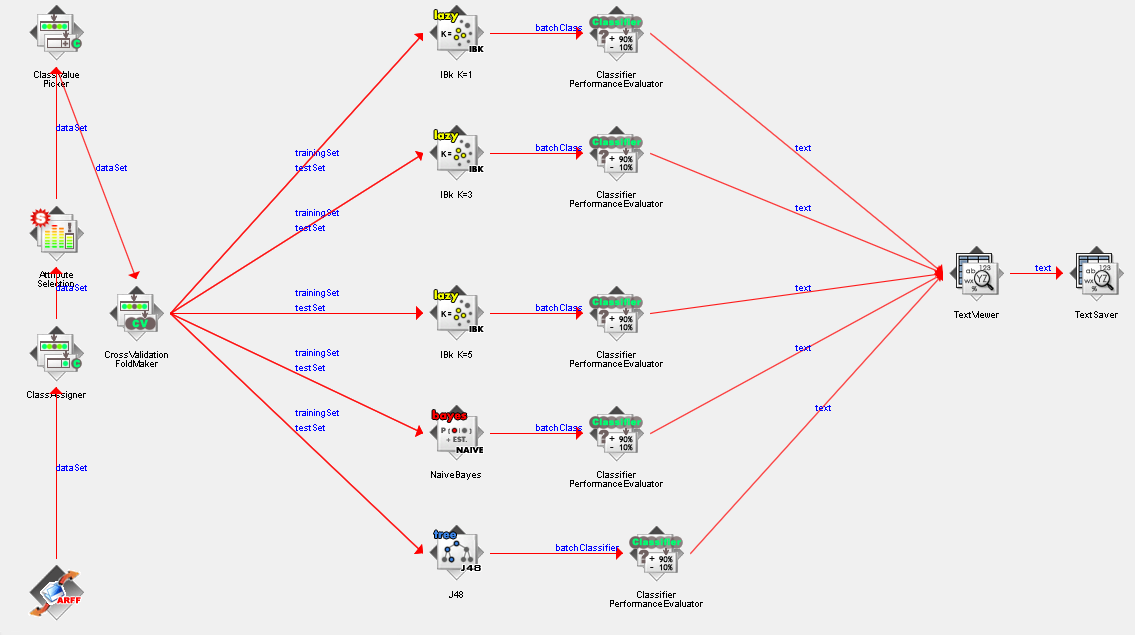
\includegraphics[width=1.4\textwidth]{./images/flow_featsel}
%\end{figure}

% \begin{sidewaysfigure}
% 	\centering
% 	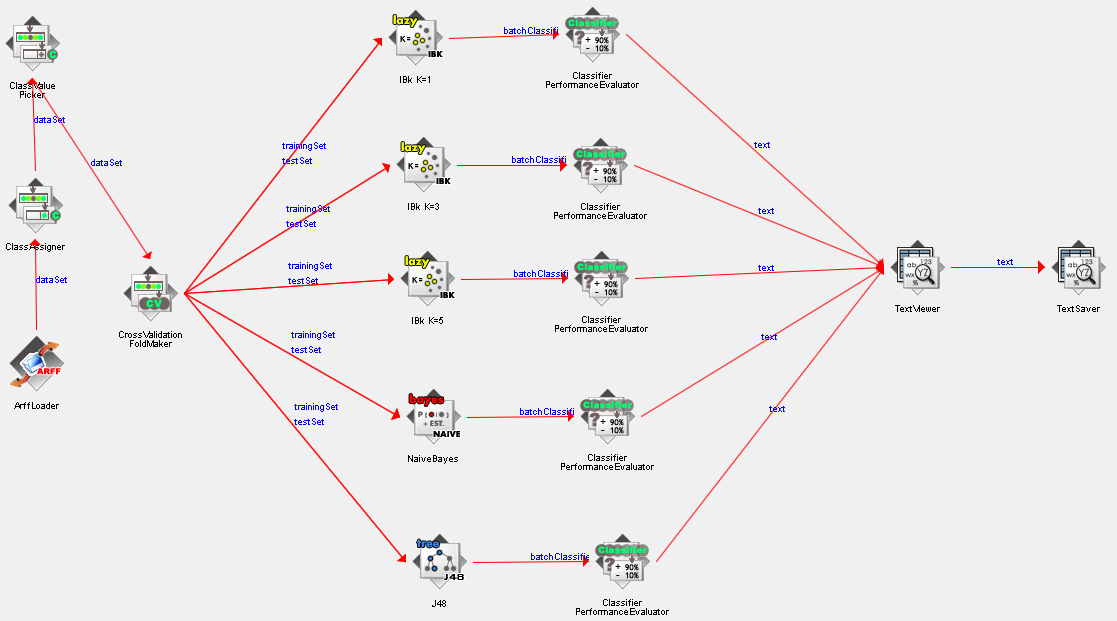
\includegraphics[width=1\textwidth]{./images/flow_no_featsel}
% \end{sidewaysfigure}

% Questo invece è lo schema con feature selection; l'unica differenza è la presenza della componente di filtraggio "AttributeSelection":

% \begin{sidewaysfigure}
% 	\centering
% 	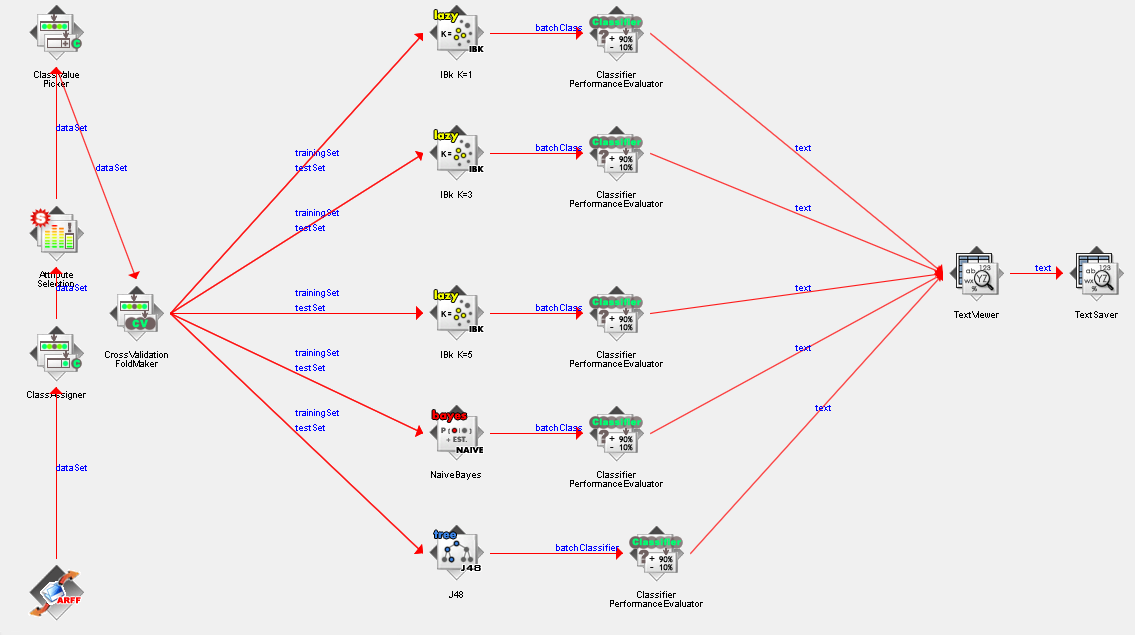
\includegraphics[width=1\textwidth]{./images/flow_featsel}
% \end{sidewaysfigure}

\subsection{Risultati delle configurazioni}
In questa sezione verranno elencati i risultati dell'esecuzione di KnowledgeFlow in base alle diverse configurazioni. \newline

%\textbf{JRip con 2 passate successive di ottimizzazione}
\vspace{0.3cm}
\begin{mdframed}[frametitle=JRip con 2 passate successive di ottimizzazione]
\begin{verbatim}
=== Evaluation result ===

Scheme: JRip #Opts: 2 : JRip
Options: -F 3 -N 2.0 -O 2 -S 1
Relation: cup98LRN


Correctly Classified Instances       16340               76.6812 %
Incorrectly Classified Instances      4969               23.3188 %
Kappa statistic                          0.5092
Mean absolute error                      0.3265
Root mean squared error                  0.4052
Relative absolute error                 65.8419 %
Root relative squared error             81.3854 %
Coverage of cases (0.95 level)          99.8123 %
Mean rel. region size (0.95 level)      88.8216 %
Total Number of Instances            21309     

=== Detailed Accuracy By Class ===

           TP Rate  FP Rate  Precision  Recall   F-Measure  ROC Area  Class
           0,492    0,004    0,990      0,492    0,657      0,746     1
           0,996    0,508    0,702      0,996    0,823      0,746     0
W. Avg.    0,767    0,279    0,833      0,767    0,748      0,746          

=== Confusion Matrix ===

a     b   <-- classified as
4766  4920 |     a = 1
49   11574 |     b = 0
\end{verbatim}
\end{mdframed}

%\textbf{JRip con 5 passate successive di ottimizzazione}

\vspace{0.5cm}
\begin{mdframed}[frametitle=JRip con 5 passate successive di ottimizzazione]
\begin{verbatim}
=== Evaluation result ===

Scheme: JRip #Opts: 5 : JRip
Options: -F 3 -N 2.0 -O 5 -S 1
Relation: cup98LRN


Correctly Classified Instances       16359               76.7704 %
Incorrectly Classified Instances      4950               23.2296 %
Kappa statistic                          0.5111
Mean absolute error                      0.3258
Root mean squared error                  0.4046
Relative absolute error                 65.7058 %
Root relative squared error             81.25   %
Coverage of cases (0.95 level)          99.8311 %
Mean rel. region size (0.95 level)      88.8193 %
Total Number of Instances            21309     

=== Detailed Accuracy By Class ===

           TP Rate  FP Rate  Precision  Recall   F-Measure  ROC Area  Class
           0,493    0,004    0,991      0,493    0,659      0,746     1
           0,996    0,507    0,702      0,996    0,824      0,746     0
W. Avg.    0,768    0,278    0,834      0,768    0,749      0,746          

=== Confusion Matrix ===

a     b   <-- classified as
4779  4907 |     a = 1
43   11580 |     b = 0
\end{verbatim}
\end{mdframed}

%\textbf{JRip con 10 passate successive di ottimizzazione}
\vspace{0.1cm}
\begin{mdframed}[frametitle=JRip con 10 passate successive di ottimizzazione]
\begin{verbatim}
=== Evaluation result ===

Scheme: JRip #Opts: 10 : JRip
Options: -F 3 -N 2.0 -O 10 -S 1
Relation: cup98LRN


Correctly Classified Instances       16374               76.8408 %
Incorrectly Classified Instances      4935               23.1592 %
Kappa statistic                          0.5126
Mean absolute error                      0.325 
Root mean squared error                  0.4042
Relative absolute error                 65.5513 %
Root relative squared error             81.1661 %
Coverage of cases (0.95 level)          99.8358 %
Mean rel. region size (0.95 level)      88.8709 %
Total Number of Instances            21309     

=== Detailed Accuracy By Class ===

           TP Rate  FP Rate  Precision  Recall   F-Measure  ROC Area  Class
           0,495    0,004    0,991      0,495    0,660      0,748     1
           0,996    0,505    0,703      0,996    0,824      0,748     0
W. Avg.    0,768    0,277    0,834      0,768    0,750      0,748          

=== Confusion Matrix ===

a     b   <-- classified as
4794  4892 |     a = 1
43   11580 |     b = 0
\end{verbatim}
\end{mdframed}

%\textbf{J48}
\vspace{0.7cm}
\begin{mdframed}[frametitle=J48 con pruning di default (EBP)]
\begin{verbatim}
=== Evaluation result ===

Scheme: J48
Options: -C 0.25 -M 2
Relation: cup98LRN


Correctly Classified Instances       14842               69.6513 %
Incorrectly Classified Instances      6467               30.3487 %
Kappa statistic                          0.3872
Mean absolute error                      0.3129
Root mean squared error                  0.524 
Relative absolute error                 63.1094 %
Root relative squared error            105.2435 %
Coverage of cases (0.95 level)          81.4398 %
Mean rel. region size (0.95 level)      65.944  %
Total Number of Instances            21309     

=== Detailed Accuracy By Class ===

           TP Rate  FP Rate  Precision  Recall   F-Measure  ROC Area  Class
           0,658    0,272    0,669      0,658    0,664      0,684     1
           0,728    0,342    0,719      0,728    0,724      0,684     0
W. Avg.    0,697    0,310    0,696      0,697    0,696      0,684          

=== Confusion Matrix ===

a    b   <-- classified as
6376 3310 |    a = 1
3157 8466 |    b = 0
\end{verbatim}
\end{mdframed}

%\textbf{J48 con pruning effettuato da REP}
\vspace{0.11cm}
\begin{mdframed}[frametitle=J48 con pruning effettuato da REP]
\begin{verbatim}
=== Evaluation result ===

Scheme: J48 w/ REP : J48
Options: -R -N 3 -Q 1 -M 2
Relation: cup98LRN


Correctly Classified Instances       16106               75.5831 %
Incorrectly Classified Instances      5203               24.4169 %
Kappa statistic                          0.4933
Mean absolute error                      0.3152
Root mean squared error                  0.4298
Relative absolute error                 63.5577 %
Root relative squared error             86.3194 %
Coverage of cases (0.95 level)          96.2457 %
Mean rel. region size (0.95 level)      84.1429 %
Total Number of Instances            21309     

=== Detailed Accuracy By Class ===

           TP Rate  FP Rate  Precision  Recall   F-Measure  ROC Area  Class
           0,562    0,083    0,850      0,562    0,677      0,762     1
           0,917    0,438    0,715      0,917    0,804      0,762     0
W. Avg.    0,756    0,276    0,776      0,756    0,746      0,762          

=== Confusion Matrix ===

a     b   <-- classified as
5448  4238 |     a = 1
965  10658 |     b = 0
\end{verbatim}
\end{mdframed}

\section{Analisi dei risultati}
Di seguito una tabella che mostra i risultati significativi delle configurazioni:

\begin{center}
\begin{tabular}{|l|c|}
	\hline
	\textbf{Configurazioni} & \textbf{Risultati} \\ \hline
	JRip con 2 passate successive di ottimizzazione (default) & 76.6812\% \\ \hline
	JRip con 5 passate successive di ottimizzazione & 76.7704\% \\ \hline
	JRip con 10 passate successive di ottimizzazione & \textbf{76.8408\%} \\ \hline
	J48 con pruning di default (EBP) & 69.6513\% \\ \hline
	J48 con pruning effettuato da REP & 75.5831\% \\ \hline
\end{tabular}
\end{center}

Come si può notare, la configurazione migliore è quella che ha previsto l'uso di JRip con 10 ottimizzazioni del ruleset con il 76.8408\% di classificazioni corrette, rispetto al 76.6812\% con solo 2 ottimizzazioni. In generale si può vedere che, ottimizzando più volte, la classificazione migliora leggermente.
Un altro aspetto interessante è dato dai risultati di J48, dove grazie al cambio del metodo di pruning, da quello di default a REP, c'è un miglioramento dal 69.6513\% al 75.5831\%, quindi un divario di quasi il 6\%, che portano la seconda configurazione di J48 ad essere competitivo con JRip.
    \clearpage
    \chapter{Deployment}
In questa fase verrà descritta una strategia di deployment, al fine di sfruttare il risultati ottenuti per motivi di business.

\section{Piano di deployment}
I risultati hanno confermato il superamento degli obiettivi di business, quindi si può utilizzare la configurazione migliore ottenuta per migliorare la predizione e l'identificazione di potenziali donatori.

\section{Monitoraggio e manutenzione}
Per assicurare un uso longevo del sistema, occorre manutenerlo raffinandolo con altri dati, provenienti da future campagne di marketing.
    \clearpage
    \bibliographystyle{abbrvnat}
    	\bibliography{mybib}
    
\end{document}